\documentclass[]{article}
\usepackage{lmodern}
\usepackage{amssymb,amsmath}
\usepackage{ifxetex,ifluatex}
\usepackage{fixltx2e} % provides \textsubscript
\ifnum 0\ifxetex 1\fi\ifluatex 1\fi=0 % if pdftex
  \usepackage[T1]{fontenc}
  \usepackage[utf8]{inputenc}
\else % if luatex or xelatex
  \ifxetex
    \usepackage{mathspec}
  \else
    \usepackage{fontspec}
  \fi
  \defaultfontfeatures{Ligatures=TeX,Scale=MatchLowercase}
\fi
% use upquote if available, for straight quotes in verbatim environments
\IfFileExists{upquote.sty}{\usepackage{upquote}}{}
% use microtype if available
\IfFileExists{microtype.sty}{%
\usepackage{microtype}
\UseMicrotypeSet[protrusion]{basicmath} % disable protrusion for tt fonts
}{}
\usepackage[margin=1in]{geometry}
\usepackage{hyperref}
\hypersetup{unicode=true,
            pdfborder={0 0 0},
            breaklinks=true}
\urlstyle{same}  % don't use monospace font for urls
\usepackage{color}
\usepackage{fancyvrb}
\newcommand{\VerbBar}{|}
\newcommand{\VERB}{\Verb[commandchars=\\\{\}]}
\DefineVerbatimEnvironment{Highlighting}{Verbatim}{commandchars=\\\{\}}
% Add ',fontsize=\small' for more characters per line
\usepackage{framed}
\definecolor{shadecolor}{RGB}{248,248,248}
\newenvironment{Shaded}{\begin{snugshade}}{\end{snugshade}}
\newcommand{\KeywordTok}[1]{\textcolor[rgb]{0.13,0.29,0.53}{\textbf{#1}}}
\newcommand{\DataTypeTok}[1]{\textcolor[rgb]{0.13,0.29,0.53}{#1}}
\newcommand{\DecValTok}[1]{\textcolor[rgb]{0.00,0.00,0.81}{#1}}
\newcommand{\BaseNTok}[1]{\textcolor[rgb]{0.00,0.00,0.81}{#1}}
\newcommand{\FloatTok}[1]{\textcolor[rgb]{0.00,0.00,0.81}{#1}}
\newcommand{\ConstantTok}[1]{\textcolor[rgb]{0.00,0.00,0.00}{#1}}
\newcommand{\CharTok}[1]{\textcolor[rgb]{0.31,0.60,0.02}{#1}}
\newcommand{\SpecialCharTok}[1]{\textcolor[rgb]{0.00,0.00,0.00}{#1}}
\newcommand{\StringTok}[1]{\textcolor[rgb]{0.31,0.60,0.02}{#1}}
\newcommand{\VerbatimStringTok}[1]{\textcolor[rgb]{0.31,0.60,0.02}{#1}}
\newcommand{\SpecialStringTok}[1]{\textcolor[rgb]{0.31,0.60,0.02}{#1}}
\newcommand{\ImportTok}[1]{#1}
\newcommand{\CommentTok}[1]{\textcolor[rgb]{0.56,0.35,0.01}{\textit{#1}}}
\newcommand{\DocumentationTok}[1]{\textcolor[rgb]{0.56,0.35,0.01}{\textbf{\textit{#1}}}}
\newcommand{\AnnotationTok}[1]{\textcolor[rgb]{0.56,0.35,0.01}{\textbf{\textit{#1}}}}
\newcommand{\CommentVarTok}[1]{\textcolor[rgb]{0.56,0.35,0.01}{\textbf{\textit{#1}}}}
\newcommand{\OtherTok}[1]{\textcolor[rgb]{0.56,0.35,0.01}{#1}}
\newcommand{\FunctionTok}[1]{\textcolor[rgb]{0.00,0.00,0.00}{#1}}
\newcommand{\VariableTok}[1]{\textcolor[rgb]{0.00,0.00,0.00}{#1}}
\newcommand{\ControlFlowTok}[1]{\textcolor[rgb]{0.13,0.29,0.53}{\textbf{#1}}}
\newcommand{\OperatorTok}[1]{\textcolor[rgb]{0.81,0.36,0.00}{\textbf{#1}}}
\newcommand{\BuiltInTok}[1]{#1}
\newcommand{\ExtensionTok}[1]{#1}
\newcommand{\PreprocessorTok}[1]{\textcolor[rgb]{0.56,0.35,0.01}{\textit{#1}}}
\newcommand{\AttributeTok}[1]{\textcolor[rgb]{0.77,0.63,0.00}{#1}}
\newcommand{\RegionMarkerTok}[1]{#1}
\newcommand{\InformationTok}[1]{\textcolor[rgb]{0.56,0.35,0.01}{\textbf{\textit{#1}}}}
\newcommand{\WarningTok}[1]{\textcolor[rgb]{0.56,0.35,0.01}{\textbf{\textit{#1}}}}
\newcommand{\AlertTok}[1]{\textcolor[rgb]{0.94,0.16,0.16}{#1}}
\newcommand{\ErrorTok}[1]{\textcolor[rgb]{0.64,0.00,0.00}{\textbf{#1}}}
\newcommand{\NormalTok}[1]{#1}
\usepackage{longtable,booktabs}
\usepackage{graphicx,grffile}
\makeatletter
\def\maxwidth{\ifdim\Gin@nat@width>\linewidth\linewidth\else\Gin@nat@width\fi}
\def\maxheight{\ifdim\Gin@nat@height>\textheight\textheight\else\Gin@nat@height\fi}
\makeatother
% Scale images if necessary, so that they will not overflow the page
% margins by default, and it is still possible to overwrite the defaults
% using explicit options in \includegraphics[width, height, ...]{}
\setkeys{Gin}{width=\maxwidth,height=\maxheight,keepaspectratio}
\IfFileExists{parskip.sty}{%
\usepackage{parskip}
}{% else
\setlength{\parindent}{0pt}
\setlength{\parskip}{6pt plus 2pt minus 1pt}
}
\setlength{\emergencystretch}{3em}  % prevent overfull lines
\providecommand{\tightlist}{%
  \setlength{\itemsep}{0pt}\setlength{\parskip}{0pt}}
\setcounter{secnumdepth}{0}
% Redefines (sub)paragraphs to behave more like sections
\ifx\paragraph\undefined\else
\let\oldparagraph\paragraph
\renewcommand{\paragraph}[1]{\oldparagraph{#1}\mbox{}}
\fi
\ifx\subparagraph\undefined\else
\let\oldsubparagraph\subparagraph
\renewcommand{\subparagraph}[1]{\oldsubparagraph{#1}\mbox{}}
\fi

%%% Use protect on footnotes to avoid problems with footnotes in titles
\let\rmarkdownfootnote\footnote%
\def\footnote{\protect\rmarkdownfootnote}

%%% Change title format to be more compact
\usepackage{titling}

% Create subtitle command for use in maketitle
\newcommand{\subtitle}[1]{
  \posttitle{
    \begin{center}\large#1\end{center}
    }
}

\setlength{\droptitle}{-2em}

  \title{}
    \pretitle{\vspace{\droptitle}}
  \posttitle{}
    \author{}
    \preauthor{}\postauthor{}
    \date{}
    \predate{}\postdate{}
  

\begin{document}

\section{brms}\label{brms}

\textbf{brms} on pakett, mis võimaldab kirjutada lihtsat süntaksit
kasutades ka üsna keerulisi mudeleid ja need Stan-is fittida. Brms on
loodud Paul Bürkneri poolt
(\url{https://github.com/paul-buerkner/brms}), mis on oma
kasutuslihtsuse tõttu jõudnud isegi ette Stani meeskonna arendatavast
analoogsest paketist \textbf{rstanarm}
(\url{https://github.com/stan-dev/rstanarm/blob/master/README.md}). Paul
Bürkner oli mõned aastad tagasi psühholoogia doktorant, kes kirjutas
brms-i algselt naljaviluks oma doktoriprojekti kõrvalt, mille tulemusel
on ta praegu teatud ringkonnis tuntum kui Lady Gaga.

\textbf{rstanarm}, mide me siin ei käsitle, püüab pakkuda tavalisete
sageduslikele meetoditele (ANOVA, lineaarne regressioon jne) bayesi
analooge, mille mudeli spetsifikatsioon ja väljund erineks võimalikult
vähe tavalisest baas-R-i töövoost. \textbf{brms} on keskendunud
mitmetasemelistele mudelitele ja kasutab põhimõtteliselt \textbf{lme4}
(\url{https://github.com/lme4/lme4/}) mudelite keelt. Loomulikult saab
\textbf{brms}-is fittida ka lineaarseid ja mitte-lineaareid
ühetasemelisi mudeleid, nagu ka imputeerida andmeid ja teha palju muud
(nagu näiteks pitsat valmistada).

\begin{Shaded}
\begin{Highlighting}[]
\KeywordTok{library}\NormalTok{(tidyverse)}
\KeywordTok{library}\NormalTok{(skimr)}
\KeywordTok{library}\NormalTok{(brms)}
\KeywordTok{library}\NormalTok{(loo)}
\KeywordTok{library}\NormalTok{(broom)}
\KeywordTok{library}\NormalTok{(bayesplot)}
\KeywordTok{library}\NormalTok{(gridExtra)}
\KeywordTok{library}\NormalTok{(mice)}
\KeywordTok{library}\NormalTok{(pROC)}
\end{Highlighting}
\end{Shaded}

\subsection{brms-i töövoog}\label{brms-i-toovoog}

\textbf{brms}-iga modelleerimisel on mõned asjad, mida tuleks teha
sõltumata sellest, millist mudelit te parajasti fitite. Kõigepealt
peaksite kontrollima, et mcmc ahelad on korralikult jooksnud (divergent
transitions, rhat ja ahelate visuaalne inspekteerimine). Lisaks peaksite
tegema posterioorse prediktiivse ploti ja vaatama, kui palju mudeli
poolt genereeritud uued valimid meenutavad teie valimit. Samuti peaksite
joonisel plottima residuaalid. Kui te inspekteerite fititud parameetrite
väärtusi, siis tehke seda posteeriorite tasemel, k.a. koos veapiiridega.
Kindlasti tuleks ka plottida mudeli ennustused koos usalduspiiridega.

Enne tõsist mudeldamist kiikame irise andmetabelisse

\begin{Shaded}
\begin{Highlighting}[]
\KeywordTok{skim}\NormalTok{(iris)}
\end{Highlighting}
\end{Shaded}

\begin{verbatim}
## Skim summary statistics
##  n obs: 150 
##  n variables: 5 
## 
## -- Variable type:factor -----------------------------------------------
##  variable missing complete   n n_unique                       top_counts
##   Species       0      150 150        3 set: 50, ver: 50, vir: 50, NA: 0
##  ordered
##    FALSE
## 
## -- Variable type:numeric ----------------------------------------------
##      variable missing complete   n mean   sd  p0 p25  p50 p75 p100
##  Petal.Length       0      150 150 3.76 1.77 1   1.6 4.35 5.1  6.9
##   Petal.Width       0      150 150 1.2  0.76 0.1 0.3 1.3  1.8  2.5
##  Sepal.Length       0      150 150 5.84 0.83 4.3 5.1 5.8  6.4  7.9
##   Sepal.Width       0      150 150 3.06 0.44 2   2.8 3    3.3  4.4
##      hist
##  ▇▁▁▂▅▅▃▁
##  ▇▁▁▅▃▃▂▂
##  ▂▇▅▇▆▅▂▂
##  ▁▂▅▇▃▂▁▁
\end{verbatim}

\begin{Shaded}
\begin{Highlighting}[]
\KeywordTok{ggplot}\NormalTok{(iris, }\KeywordTok{aes}\NormalTok{(Petal.Length, Sepal.Length)) }\OperatorTok{+}\StringTok{ }
\StringTok{  }\KeywordTok{geom_point}\NormalTok{(}\KeywordTok{aes}\NormalTok{(}\DataTypeTok{color =}\NormalTok{ Species)) }\OperatorTok{+}
\StringTok{  }\KeywordTok{geom_smooth}\NormalTok{(}\DataTypeTok{method =} \StringTok{"loess"}\NormalTok{, }\DataTypeTok{color =} \StringTok{"black"}\NormalTok{) }\OperatorTok{+}
\StringTok{  }\KeywordTok{geom_smooth}\NormalTok{(}\DataTypeTok{method =} \StringTok{"lm"}\NormalTok{)}
\end{Highlighting}
\end{Shaded}

\includegraphics{17_brms_files/figure-latex/unnamed-chunk-130-1.pdf}

Loess fit viitab, et 3 liiki ühe sirgega mudeldada pole võib-olla
optimaalne lahendus.

\begin{Shaded}
\begin{Highlighting}[]
\KeywordTok{ggplot}\NormalTok{(iris, }\KeywordTok{aes}\NormalTok{(Petal.Length, Sepal.Length, }\DataTypeTok{color =}\NormalTok{ Species)) }\OperatorTok{+}\StringTok{ }
\StringTok{  }\KeywordTok{geom_point}\NormalTok{() }\OperatorTok{+}
\StringTok{  }\KeywordTok{geom_smooth}\NormalTok{(}\DataTypeTok{method =} \StringTok{"loess"}\NormalTok{, }\KeywordTok{aes}\NormalTok{(}\DataTypeTok{group =}\NormalTok{ Species), }\DataTypeTok{color =} \StringTok{"black"}\NormalTok{) }\OperatorTok{+}
\StringTok{  }\KeywordTok{geom_smooth}\NormalTok{(}\DataTypeTok{method =} \StringTok{"lm"}\NormalTok{)}
\end{Highlighting}
\end{Shaded}

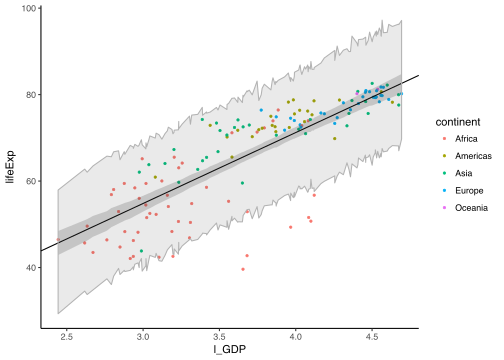
\includegraphics{17_brms_files/figure-latex/unnamed-chunk-131-1.pdf}

Nüüd on loess ja lm heas kooskõlas - seos y\textasciitilde{}x vahel
oleks nagu enam-vähem lineaarne. Siit tuleb ka välja, et kolme mudeli
tõusud on sarnased, interceptid erinevad.

\subsubsection{Kiire töövoog}\label{kiire-toovoog}

Minimaalses töövoos anname ette võimalikult vähe parameetreid ja töötame
mudeliga nii vähe kui võimalik. See on mõeldud ülevaatena Bayesi mudeli
fittimise põhilistest etappidest

Mudeli fittimine:

\begin{Shaded}
\begin{Highlighting}[]
\NormalTok{m_kiire <-}\StringTok{ }\KeywordTok{brm}\NormalTok{(Sepal.Length }\OperatorTok{~}\StringTok{ }\NormalTok{Petal.Length, }\DataTypeTok{data =}\NormalTok{ iris)}
\KeywordTok{write_rds}\NormalTok{(m_kiire, }\DataTypeTok{path =} \StringTok{"data/m_kiire.fit"}\NormalTok{)}
\end{Highlighting}
\end{Shaded}

Priorid on brms-i poolt ette antud ja loomulikult ei sisalda mingit
teaduslikku informatsiooni. Nad on siiski ``nõrgalt informatiivsed''
selles mõttes, et kasutavad parametriseeringuid, mis enamasti
võimaldavad mcmc ahelatel normaalselt joosta. Järgmises ptk-s õpime ise
prioreid määrama.

Posteeriorid ja mcmc ahelate konvergents

\begin{Shaded}
\begin{Highlighting}[]
\KeywordTok{plot}\NormalTok{(m_kiire)}
\end{Highlighting}
\end{Shaded}

\includegraphics{17_brms_files/figure-latex/unnamed-chunk-134-1.pdf}

Fiti kokkuvõte - koefitsiendid ja nende fittimise edukust hindavad
statistikud (Eff.Sample, Rhat)

\begin{Shaded}
\begin{Highlighting}[]
\KeywordTok{tidy}\NormalTok{(m_kiire)}
\end{Highlighting}
\end{Shaded}

\begin{verbatim}
##             term    estimate  std.error       lower       upper
## 1    b_Intercept   4.3069542 0.07800007   4.1792947   4.4343652
## 2 b_Petal.Length   0.4088872 0.01872377   0.3790367   0.4393033
## 3          sigma   0.4110973 0.02428369   0.3734732   0.4528043
## 4           lp__ -85.3383596 1.21734294 -87.7573958 -84.0152351
\end{verbatim}

Eff.Sample näitab efektiivset valimi suurust, mida ahelad on kasutanud.
See on suht keeruline mõiste, aga piisab, kui aru saada, et see näitaja
ei tohiks olla madalam kui paarkümmend.

Rhat on statistik, mis vaatab ahelate konvergentsi. Kui Rhat
\textgreater{} 1.1, siis on kuri karjas. Rhat 1.0 ei tähenda paraku, et
võiks rahulikult hingata -- tegu on statistikuga, mida saab hästi
tõlgendada häda kuulutajana, aga liiga sageli mitte vastupidi.

Ennustav plot ehk \emph{marginal plot} -- mudeli fit 95\% CI-ga.

\begin{Shaded}
\begin{Highlighting}[]
\KeywordTok{plot}\NormalTok{(}\KeywordTok{marginal_effects}\NormalTok{(m_kiire), }\DataTypeTok{points =} \OtherTok{TRUE}\NormalTok{)}
\end{Highlighting}
\end{Shaded}

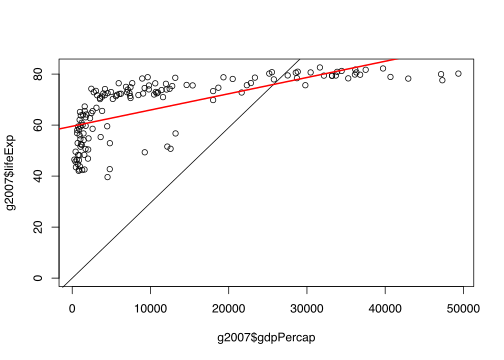
\includegraphics{17_brms_files/figure-latex/unnamed-chunk-136-1.pdf}

\subsubsection{Põhjalikum töövoog}\label{pohjalikum-toovoog}

Põhiline erinevus eelmisega on suurem tähelepanu prioritele, mudeli
fittimise diagnostikale ning tööle fititud mudeliga.

\subsubsection{Spetsifitseerime mudeli, vaatame ja muudame
vaikeprioreid}\label{spetsifitseerime-mudeli-vaatame-ja-muudame-vaikeprioreid}

brms-i default priorid on konstrueeritud olema üsna väheinformatiivsed
ja need tuleks enamasti informatiivsematega asendada. Igasse priorisse
tuleks panna nii palju informatsiooni, kui teil on vastava parameetri
kohta. Kui te mõne parameetri kohta ei oska öelda, milllised oleks selle
mõistlikud oodatavad väärtused, siis saab piirduda brms-i antud
vaikeväärtustega. Samas, kui keerulisemad mudelid ei taha hästi joosta
(mida tuleb ikka ette), siis aitab sageli priorite kitsamaks muutmine.

\begin{Shaded}
\begin{Highlighting}[]
\KeywordTok{get_prior}\NormalTok{(Sepal.Length }\OperatorTok{~}\StringTok{ }\NormalTok{Petal.Length }\OperatorTok{+}\StringTok{ }\NormalTok{(}\DecValTok{1} \OperatorTok{|}\StringTok{ }\NormalTok{Species), }
          \DataTypeTok{data =}\NormalTok{ iris)}
\end{Highlighting}
\end{Shaded}

\begin{verbatim}
##                 prior     class         coef   group resp dpar nlpar bound
## 1                             b                                           
## 2                             b Petal.Length                              
## 3 student_t(3, 6, 10) Intercept                                           
## 4 student_t(3, 0, 10)        sd                                           
## 5                            sd              Species                      
## 6                            sd    Intercept Species                      
## 7 student_t(3, 0, 10)     sigma
\end{verbatim}

Me fitime pedagoogilistel kaalutlustel shrinkage mudeli, mis tõmbab 3
liigi lõikepunkte natuke keskmise lõikepunkti suunas. On vaieldav, kas
see on irise andmestiku juures mõistlik strateegia, aga me teeme seda
siin ikkagi.

\begin{quote}
Mitmetasemeline shrinkage mudel on abinõu ülefittimise vastu. Mudelite
võrdlemisel otsitakse kompromissi - ehk mudeli, mille ennustused oleks
andmepunktidele võimalikult lähedal ilma,et see mudel oleks liiga
keeruliseks aetud (keerulisus on proportsionaalne mudeli parameetrite
arvuga).
\end{quote}

Prioreid muudame nii:

\begin{Shaded}
\begin{Highlighting}[]
\NormalTok{prior <-}\StringTok{ }\KeywordTok{c}\NormalTok{(}\KeywordTok{prior}\NormalTok{(}\KeywordTok{normal}\NormalTok{(}\DecValTok{6}\NormalTok{, }\DecValTok{3}\NormalTok{), }\DataTypeTok{class =} \StringTok{"Intercept"}\NormalTok{),}
           \KeywordTok{prior}\NormalTok{(}\KeywordTok{normal}\NormalTok{(}\DecValTok{0}\NormalTok{, }\DecValTok{1}\NormalTok{), }\DataTypeTok{class =} \StringTok{"b"}\NormalTok{),}
           \KeywordTok{prior}\NormalTok{(}\KeywordTok{student_t}\NormalTok{(}\DecValTok{6}\NormalTok{, }\DecValTok{0}\NormalTok{, }\DecValTok{2}\NormalTok{), }\DataTypeTok{class =} \StringTok{"sigma"}\NormalTok{))}
\end{Highlighting}
\end{Shaded}

Me valime siin nn väheinformariivsed priorid, nii et regressiooni
tulemus on suht hästi võrreldav lme4 sagedusliku mudeliga. ``b''
koefitsiendi priorile (aga mitte ``sigma'' ega ``Intercept''-le) võib
anda ka ülemise ja/või alumise piiri
\texttt{prior(normal(0,\ 1),\ class\ =\ "b",\ lb\ =\ -1,\ ub\ =\ 10)}
ütleb, et ``b'' prior on nullist erinev ainult -1 ja 10 vahel. ``sigma''
priorid on automaatselt lb = 0-ga, sest varieeruvus ei tohi olla
negatiivne.

Alati tasub prioreid pildil vaadata, et veenduda nende mõistlikuses.

\begin{Shaded}
\begin{Highlighting}[]
\NormalTok{x <-}\StringTok{ }\KeywordTok{seq}\NormalTok{(}\DecValTok{0}\NormalTok{, }\DecValTok{10}\NormalTok{, }\DataTypeTok{length.out =} \DecValTok{100}\NormalTok{)}
\NormalTok{y <-}\StringTok{ }\KeywordTok{dstudent_t}\NormalTok{(x, }\DataTypeTok{df =} \DecValTok{6}\NormalTok{, }\DataTypeTok{mu =} \DecValTok{0}\NormalTok{, }\DataTypeTok{sigma =} \DecValTok{2}\NormalTok{, }\DataTypeTok{log =} \OtherTok{FALSE}\NormalTok{)}
\KeywordTok{plot}\NormalTok{(y }\OperatorTok{~}\StringTok{ }\NormalTok{x)}
\end{Highlighting}
\end{Shaded}

\includegraphics{17_brms_files/figure-latex/unnamed-chunk-139-1.pdf}
Sigma prior, mida \textbf{brms} kasutab, on vaikimisi pool
sümmeetrilisest jaotusest, mis lõigatakse nulli kohalt pooleks nii, et
seal puuduvad \textless{} 0 väärtused (seega ei saa varieeruvuse
posteerior minna alla nulli).

Me võime ka prioreid ilma likelihoodideta (tõepärafunktsioonideta) läbi
mudeli lasta, misjärel tõmbame fititud mudelist priorite valimid (neid
võiks kutsuda ka ``priorite posteerioriteks'') ja plotime kõik priorid
koos. Seda pilti saab siis võrrelda koos andmetega fititud mudeli
posteerioritega. Selle võimaluse kasutamine on tõusuteel, sest
keerulisemate mudelite puhul võib priorite ükshaaval plottimine osutuda
eksitavaks.

Tekitame priorite valimid, et näha oma priorite mõistlikust (brm()
argument on sample\_prior = TRUE). Ühtlasi fitime ka oma mudeli koos
andmete ja prioritega.

\begin{Shaded}
\begin{Highlighting}[]
\NormalTok{m1 <-}\StringTok{ }\KeywordTok{brm}\NormalTok{(Sepal.Length }\OperatorTok{~}\StringTok{ }\NormalTok{Petal.Length }\OperatorTok{+}\StringTok{ }\NormalTok{(}\DecValTok{1} \OperatorTok{|}\StringTok{ }\NormalTok{Species), }
          \DataTypeTok{data =}\NormalTok{ iris, }
          \DataTypeTok{prior =}\NormalTok{ prior, }
          \DataTypeTok{family =}\NormalTok{ gaussian,}
          \DataTypeTok{warmup =} \DecValTok{1000}\NormalTok{,}
          \DataTypeTok{iter =} \DecValTok{2000}\NormalTok{,}
          \DataTypeTok{chains =} \DecValTok{3}\NormalTok{,}
          \DataTypeTok{cores =} \DecValTok{3}\NormalTok{,}
          \DataTypeTok{sample_prior =} \OtherTok{TRUE}\NormalTok{)}
\KeywordTok{write_rds}\NormalTok{(m1, }\DataTypeTok{path =} \StringTok{"data/m1.fit"}\NormalTok{)}
\end{Highlighting}
\end{Shaded}

Me fittisime mudeli m1 kaks korda: nii andmetega (selle juurde jõuame
varsti), kui ka ilma andmeteta. Kui panna sisse
\texttt{sample\_prior\ =\ "only"}, siis jookseb mudel ilma andmeteta, ja
selle võrra kiiremini. Vaikeväärtus on \texttt{sample\_prior\ =\ "no"},
mis tähendab, et fititakse ainult üks mudel - koos andmetega. Ilma
andmeteta (likelihoodita) fitist saame tõmmata priorite mcmc valimid,
mille ka järgmiseks plotime.

\begin{Shaded}
\begin{Highlighting}[]
\KeywordTok{prior_samples}\NormalTok{(m1) }\OperatorTok\StringTok{ }
\StringTok{  }\KeywordTok{gather}\NormalTok{() }\OperatorTok\StringTok{ }
\StringTok{  }\KeywordTok{ggplot}\NormalTok{() }\OperatorTok{+}\StringTok{ }
\StringTok{  }\KeywordTok{geom_density}\NormalTok{(}\KeywordTok{aes}\NormalTok{(value)) }\OperatorTok{+}\StringTok{ }
\StringTok{  }\KeywordTok{facet_wrap}\NormalTok{(}\OperatorTok{~}\StringTok{ }\NormalTok{key, }\DataTypeTok{scales =} \StringTok{"free_x"}\NormalTok{)}
\end{Highlighting}
\end{Shaded}

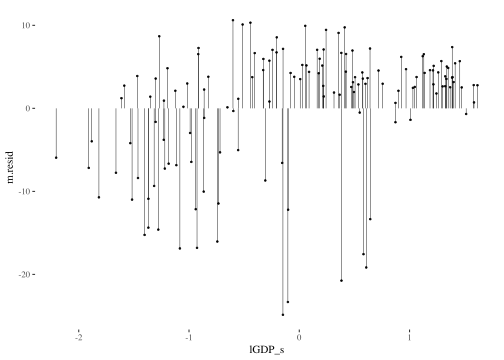
\includegraphics{17_brms_files/figure-latex/unnamed-chunk-142-1.pdf}

Kui kasutame \texttt{sample\_prior\ =\ "only"} varianti, siis on esimene
koodirida erinev: \texttt{samples1\ =\ as.data.frame(m1\$fit)}.

\begin{quote}
\textbf{brms}-i Intercepti priorite spetsifitseerimisel tasub teada, et
\textbf{brms} oma sisemuses tsentreerib kõik prediktorid nullile (x -
mean(x)), ja teie poolt ette antud prior peaks vastama neile
tsentreeritud prediktoritele, kus kõikide prediktorite keskväärtus on
null. Põhjus on, et tsentreeritud parametriseeringuga mudelid jooksevad
sageli paremini. Alternatiiv on kasutada mudeli tavapärase süntaksi y
\textasciitilde{} 1 + x (või ekvivalentselt y \textasciitilde{} x)
asemel süntaksit y \textasciitilde{} 0 + intercept + x. Sellisel juhul
saab anda priorid tsentreerimata predikroritele. Lisaks on \textbf{brms}
selle süntaksi puhul nõus ``b''-le antud prioreid vaikimisi ka
intercepti fittimisel kasutama.
\end{quote}

\subsubsection{\texorpdfstring{\texttt{brm()} funktsiooni
argumendid:}{brm() funktsiooni argumendid:}}\label{brm-funktsiooni-argumendid}

\begin{itemize}
\item
  family - tõepärafunktsiooni tüüp (modelleerib y muutuja jaotust e
  likelihoodi)
\item
  warmup - mitu sammu mcmc ahel astub, enne kui ahelat salvestama
  hakatakse. tavaliselt on 500-1000 sammu piisav, et tagada ahelate
  konvergents. Kui ei ole, tõstke 2000 sammuni.
\item
  iter - ahelate sammude arv, mida salvestatakse peale warmup perioodi.
  Enamasti on 2000 piisav. Kui olete nõus piirduma posteeriori
  keskväärtuse arvutamisega ja ei soovi täpseid usaldusintervalle, siis
  võib piisata ka 200 sammust.
\item
  chains - mitu sõltumatut mcmc ahelat jooksutada. 3 on hea selleks, et
  näha kas ahelad konvergeeruvad. Kui mitte, tuleks lisada
  informatiivsemaid prioreid ja/või warmupi pikkust.
\item
  cores - mitu teie arvuti tuuma ahelaid jooksutama panna.
\item
  adapt\_delta - mida suurem number (max = 1), seda stabiilsemalt, ja
  aeglasemalt, ahelad jooksevad.
\item
  thin - kui ahel on autokorreleeritud, st ahela eelmine samm suudab
  ennustada järgevaid (see on paha), siis saab salvestada näit ahela iga
  5. sammu (thin = 5). Aga siis tuleks ka sammude arvu 5 korda tõsta.
  Vaikeväärtus on thin = 1. Autokorrelatsiooni graafilist määramist
  näitame allpool
\end{itemize}

Järgmine funktsioon trükib välja Stani koodi, mis spetsifitseerib
mudeli, mida tegelikult Stanis fittima hakatakse. See on väga kasulik,
aga ainult siis kui tahate õppida otse Stanis mudeleid kirjutama:

\begin{Shaded}
\begin{Highlighting}[]
\KeywordTok{make_stancode}\NormalTok{(Sepal.Length }\OperatorTok{~}\StringTok{ }\NormalTok{Petal.Length, }\DataTypeTok{data =}\NormalTok{ iris, }\DataTypeTok{prior =}\NormalTok{ prior)}
\end{Highlighting}
\end{Shaded}

\subsubsection{Fitime mudeleid ja võrdleme
fitte.}\label{fitime-mudeleid-ja-vordleme-fitte.}

Eelmises mudelis (m1) ennustame muutuja Sepal.Length väärtusi
Petal.Length väärtuste põhjal shrinkage mudelis, kus iga irise liik on
oma grupis.

Teine mudel, mis sisaldab veel üht ennustavat muutujat (Sepal.Width):

\begin{Shaded}
\begin{Highlighting}[]
\NormalTok{m2 <-}\StringTok{ }\KeywordTok{brm}\NormalTok{(Sepal.Length }\OperatorTok{~}\StringTok{ }\NormalTok{Petal.Length }\OperatorTok{+}\StringTok{ }\NormalTok{Sepal.Width }\OperatorTok{+}\StringTok{ }\NormalTok{(}\DecValTok{1} \OperatorTok{|}\StringTok{ }\NormalTok{Species), }
          \DataTypeTok{data =}\NormalTok{ iris, }
          \DataTypeTok{prior =}\NormalTok{ prior)}
\KeywordTok{write_rds}\NormalTok{(m2, }\DataTypeTok{path =} \StringTok{"data/m2.fit"}\NormalTok{)}
\end{Highlighting}
\end{Shaded}

Kolmandaks ühetasemeline mudel, mis vaatab kolme irise liiki eraldi:

\begin{Shaded}
\begin{Highlighting}[]
\NormalTok{m3 <-}\StringTok{ }\KeywordTok{brm}\NormalTok{(Sepal.Length }\OperatorTok{~}\StringTok{ }\NormalTok{Sepal.Width }\OperatorTok{+}\StringTok{ }\NormalTok{Petal.Length }\OperatorTok{*}\StringTok{ }\NormalTok{Species, }
          \DataTypeTok{data =}\NormalTok{ iris, }
          \DataTypeTok{prior =}\NormalTok{ prior)}
\KeywordTok{write_rds}\NormalTok{(m3, }\DataTypeTok{path =} \StringTok{"data/m3.fit"}\NormalTok{)}
\end{Highlighting}
\end{Shaded}

Ja lõpuks mudel, mis paneb kõik liigid ühte patta:

\begin{Shaded}
\begin{Highlighting}[]
\NormalTok{m4 <-}\StringTok{ }\KeywordTok{brm}\NormalTok{(Sepal.Length }\OperatorTok{~}\StringTok{ }\NormalTok{Petal.Length }\OperatorTok{+}\StringTok{ }\NormalTok{Sepal.Width, }
          \DataTypeTok{data =}\NormalTok{ iris, }
          \DataTypeTok{prior =}\NormalTok{ prior)}
\KeywordTok{write_rds}\NormalTok{(m4, }\DataTypeTok{path =} \StringTok{"data/m4.fit"}\NormalTok{)}
\end{Highlighting}
\end{Shaded}

Siin me võrdleme neid nelja mudelit. Väikseim looic (leave-one-out
information criterion) võidab. See on suhteline võrdlus -- looic abs
väärtus ei mängi mingit rolli.

\begin{Shaded}
\begin{Highlighting}[]
\KeywordTok{loo}\NormalTok{(m1, m2, m3, m4)}
\end{Highlighting}
\end{Shaded}

\begin{verbatim}
##          LOOIC    SE
## m1      106.43 16.65
## m2       81.61 16.11
## m3       80.06 15.77
## m4      100.55 16.41
## m1 - m2  24.82  9.63
## m1 - m3  26.37 10.66
## m1 - m4   5.88 15.28
## m2 - m3   1.55  3.34
## m2 - m4 -18.94  9.90
## m3 - m4 -20.49  9.95
\end{verbatim}

Siin on m1 ja m2/m3 mudeli erinevus 25 ühikut ja selle erinevuse
standardviga on 10 ühikut. 2 SE-d annab umbkaudu 95\% usaldusintervalli,
ja see ei kata antud juhul nulli. Seega järeldame, et m2 ja m3, mis
kasutavad ennustamiseks lisamuutujat, on selgelt eelistatud. Samas ei
saa me õelda, et hierarhiline mudel m2 oleks parem või halvem kui
interaktsioonimudel m3. Ka puudub oluline erinevus m1 ja m4 fiti vahel.
Tundub, et selle ennustusjõu, mille me võidame lisaparameetrit
mudeldades, kaotame omakorda liike ühte patta pannes (neid mitte
osaliselt iseseisvana modelleerides).

Alternatiivina kasutame \texttt{brms::waic} kriteeriumit mudelite
võrdlemiseks. See töötab kiiremini kui LOO ja tõlgendus on sarnane -
väikseim waic võidab ja absolutväärtusi ei saa ükshaaval tõlgendada.

\begin{Shaded}
\begin{Highlighting}[]
\KeywordTok{waic}\NormalTok{(m1, m2, m3, m4)}
\end{Highlighting}
\end{Shaded}

\begin{verbatim}
##           WAIC    SE
## m1      106.40 16.64
## m2       81.55 16.10
## m3       79.96 15.76
## m4      100.53 16.41
## m1 - m2  24.85  9.63
## m1 - m3  26.44 10.67
## m1 - m4   5.87 15.28
## m2 - m3   1.60  3.34
## m2 - m4 -18.98  9.90
## m3 - m4 -20.57  9.95
\end{verbatim}

Nagu näha, annavad LOO ja waic sageli väga sarnaseid tulemusi.

Me ei süvene LOOIC ega waic-i statistilisse mõttesse, sest bayesi
mudelite võrdlemine on kiiresti arenev ala, kus ühte parimat lahendust
pole veel leitud.

\subsubsection{Vaatame mudelite
kokkuvõtet}\label{vaatame-mudelite-kokkuvotet}

Lihtne tabel mudeli m2 fititud koefitsientidest koos 95\%
usalduspiiridega

\begin{Shaded}
\begin{Highlighting}[]
\KeywordTok{tidy}\NormalTok{(m2)}
\end{Highlighting}
\end{Shaded}

\begin{verbatim}
##                              term    estimate  std.error        lower
## 1                     b_Intercept   1.7103643 1.02696434   0.09501731
## 2                  b_Petal.Length   0.7586935 0.06447171   0.65102517
## 3                   b_Sepal.Width   0.4399983 0.08390346   0.30344396
## 4           sd_Species__Intercept   1.7245533 1.53152570   0.43254413
## 5                           sigma   0.3133531 0.01858008   0.28372899
## 6     r_Species[setosa,Intercept]   0.6761215 0.99251544  -0.90137958
## 7 r_Species[versicolor,Intercept]  -0.2256225 0.98418414  -1.85304215
## 8  r_Species[virginica,Intercept]  -0.6421414 0.99073910  -2.27687000
## 9                            lp__ -50.4332187 2.36799011 -54.78758033
##         upper
## 1   3.3445499
## 2   0.8657980
## 3   0.5757067
## 4   5.0237993
## 5   0.3454901
## 6   2.2495333
## 7   1.2525412
## 8   0.8091602
## 9 -47.1687175
\end{verbatim}

r\_ prefiks tähendab, et antud koefitsient kuulub mudeli esimesele
(madalamale) tasemele (Liigi tase) r - random - tähendab, et iga grupi
(liigi) sees arvutatakse oma fit. b\_ tähendab mudeli 2. taset
(keskmistatud üle kõikide gruppide). 2. tasmel on meil intercept, b1 ja
b2 tõusud ning standardhälve y muutuja ennustatud andempunktide tasemel.
1. tasemel on meil 3 liigi interceptide erinevus üldisest b\_Intercepti
väärtusest. Seega, selleks, et saada setosa liigi intercepti, peame
tegema tehte 1.616 + 0.765.

\textbf{tidy} funktsiooni tööd saab kontrollida järgmiste parameetrite
abil:

\begin{Shaded}
\begin{Highlighting}[]
\KeywordTok{tidy}\NormalTok{(x, }\DataTypeTok{parameters =} \OtherTok{NA}\NormalTok{, }\DataTypeTok{par_type =} \KeywordTok{c}\NormalTok{(}\StringTok{"all"}\NormalTok{,}
  \StringTok{"non-varying"}\NormalTok{, }\StringTok{"varying"}\NormalTok{, }\StringTok{"hierarchical"}\NormalTok{), }\DataTypeTok{robust =} \OtherTok{FALSE}\NormalTok{,}
  \DataTypeTok{intervals =} \OtherTok{TRUE}\NormalTok{, }\DataTypeTok{prob =} \FloatTok{0.9}\NormalTok{, ...)}
\end{Highlighting}
\end{Shaded}

par\_type = ``hierarchical'' kuvab grupi taseme parameetrite sd-d ja
korrelatsioonid. ``varying'' kuvab grupi taseme interceptid ja tõusud
(siis kui neid mudeldadakse). ``non-varying'' kuvab kõrgema taseme
(grupi-ülesed) parameetrid. robust = TRUE annab estimate posteeriori
mediaanina (vaikeväärtus FALSE annab selle aritmeetilise keskmisena
posteeriorist).

Nüüd põhjalikum mudeli kokkuvõte:

\begin{Shaded}
\begin{Highlighting}[]
\NormalTok{m2}
\end{Highlighting}
\end{Shaded}

\begin{verbatim}
## Warning: There were 17 divergent transitions after warmup. Increasing adapt_delta above 0.95 may help.
## See http://mc-stan.org/misc/warnings.html#divergent-transitions-after-warmup
\end{verbatim}

\begin{verbatim}
##  Family: gaussian 
##   Links: mu = identity; sigma = identity 
## Formula: Sepal.Length ~ Petal.Length + Sepal.Width + (1 | Species) 
##    Data: iris (Number of observations: 150) 
## Samples: 3 chains, each with iter = 2000; warmup = 1000; thin = 1;
##          total post-warmup samples = 3000
## 
## Group-Level Effects: 
## ~Species (Number of levels: 3) 
##               Estimate Est.Error l-95% CI u-95% CI Eff.Sample Rhat
## sd(Intercept)     1.72      1.53     0.36     5.98        503 1.00
## 
## Population-Level Effects: 
##              Estimate Est.Error l-95% CI u-95% CI Eff.Sample Rhat
## Intercept        1.71      1.03    -0.36     4.08        550 1.01
## Petal.Length     0.76      0.06     0.63     0.88       1380 1.00
## Sepal.Width      0.44      0.08     0.27     0.60       1857 1.00
## 
## Family Specific Parameters: 
##       Estimate Est.Error l-95% CI u-95% CI Eff.Sample Rhat
## sigma     0.31      0.02     0.28     0.35       1882 1.00
## 
## Samples were drawn using sampling(NUTS). For each parameter, Eff.Sample 
## is a crude measure of effective sample size, and Rhat is the potential 
## scale reduction factor on split chains (at convergence, Rhat = 1).
\end{verbatim}

Siin on eraldi toodud grupi tasemel ja populatsiooni tasemel
koefitsiendid ja gruppide vaheline sd (= 1.72). Pane tähele, et üldine
varieeruvus sigma = 0.31 on palju väiksem kui gruppide vaheline
varieeruvus sd(Intercept) = 1.72. Seega on grupid üksteisest tugevalt
erinevad ja neid tuleks võib-olla tõesti eraldi modelleerida.

Divergentsed transitsioonid on halvad asjad - ahelad on läinud 17 korda
metsa. Viisakas oleks adapt deltat tõsta või kitsamad priorid panna, aga
17 halba andmepunkti paarist tuhandest, mille mcmc ahelad meile
tekitasid, pole ka mingi maailmalõpp. Nii et las praegu jääb nagu on.
Need divergentsed transitsioonid on kerged tekkima just
mitmetasemelistes mudelites.

\subsubsection{Plotime posteeriorid ja
ahelad}\label{plotime-posteeriorid-ja-ahelad}

\begin{Shaded}
\begin{Highlighting}[]
\KeywordTok{plot}\NormalTok{(m2)}
\end{Highlighting}
\end{Shaded}

\includegraphics{17_brms_files/figure-latex/unnamed-chunk-153-1.pdf}

Siit on näha, et ahelad on ilusti konvergeerunud. Ühtlasi on pildil
posterioorsed jaotused fititud koefitsientidele.

\emph{Regular expressioni} abil saab plottida mudeli madalama taseme
ahelaid \& posteerioreid, mida plot() vaikimisi ei näita.

\begin{Shaded}
\begin{Highlighting}[]
\KeywordTok{plot}\NormalTok{(m2, }\DataTypeTok{pars =} \StringTok{"r_"}\NormalTok{)}
\end{Highlighting}
\end{Shaded}

\includegraphics{17_brms_files/figure-latex/unnamed-chunk-154-1.pdf}

Vaatame korrelatsioone erinevate parameetrite posterioorsete valimite
vahel. (Markovi ahelad jooksevad n-mõõtmelises ruumis, kus n on mudeli
parameetrite arv, mille väärtusi hinnatakse.) Pairs(m3) teeb pildi ära,
aga ilusama pildi saab \texttt{GGally::ggpairs()} abil.

\begin{Shaded}
\begin{Highlighting}[]
\KeywordTok{pairs}\NormalTok{(m2, }\DataTypeTok{pars =} \StringTok{"b_"}\NormalTok{)}
\end{Highlighting}
\end{Shaded}

\includegraphics{17_brms_files/figure-latex/unnamed-chunk-155-1.pdf}

\begin{Shaded}
\begin{Highlighting}[]
\KeywordTok{library}\NormalTok{(GGally)}
\KeywordTok{posterior_samples}\NormalTok{(m2) }\OperatorTok
\StringTok{  }\KeywordTok{select}\NormalTok{(}\KeywordTok{contains}\NormalTok{(}\StringTok{"b_"}\NormalTok{)) }\OperatorTok
\StringTok{  }\KeywordTok{ggpairs}\NormalTok{()}
\end{Highlighting}
\end{Shaded}

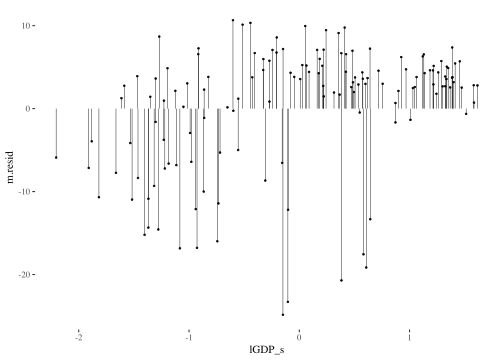
\includegraphics{17_brms_files/figure-latex/unnamed-chunk-156-1.pdf}

Siin on posteeriorite põhjal arvutatud 50\% ja 95\% CI ja see plotitud.

\begin{Shaded}
\begin{Highlighting}[]
\KeywordTok{stanplot}\NormalTok{(m2, }\DataTypeTok{pars =} \StringTok{"r_"}\NormalTok{, }\DataTypeTok{type =} \StringTok{"intervals"}\NormalTok{)}
\end{Highlighting}
\end{Shaded}

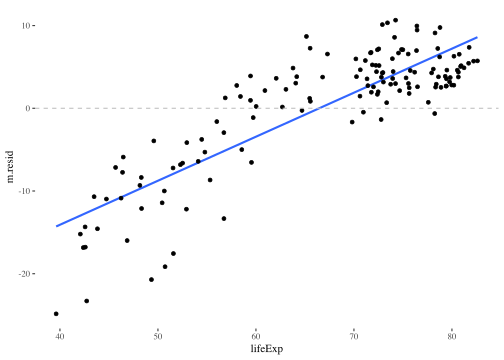
\includegraphics{17_brms_files/figure-latex/unnamed-chunk-157-1.pdf}

type = argument sisestamine võimaldab plottida erinevaid diagnostilisi
näitajaid. Lubatud sisendid on ``hist'', ``dens'', ``hist\_by\_chain'',
``dens\_overlay'', ``violin'', ``intervals'', ``areas'', ``acf'',
``acf\_bar'', ``trace'', ``trace\_highlight'', ``scatter'', ``rhat'',
``rhat\_hist'', ``neff'', ``neff\_hist'' ``nuts\_acceptance'',
``nuts\_divergence'', ``nuts\_stepsize'', ``nuts\_treedepth'' ja
``nuts\_energy''.

\begin{Shaded}
\begin{Highlighting}[]
\KeywordTok{stanplot}\NormalTok{(m2, }\DataTypeTok{type =} \StringTok{"neff"}\NormalTok{)}
\end{Highlighting}
\end{Shaded}

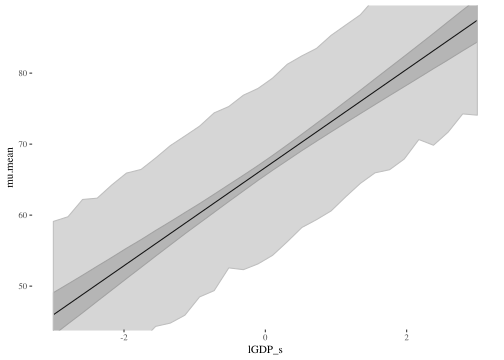
\includegraphics{17_brms_files/figure-latex/unnamed-chunk-158-1.pdf}

Neff on efektiivne valimi suurus ja senikaua kuni Neff/N suhe ei ole
\textless{} 0.1, pole põhjust selle pärast muretseda.

\subsubsection{Korjame ahelad andmeraami ja plotime fititud
koefitsiendid
CI-dega}\label{korjame-ahelad-andmeraami-ja-plotime-fititud-koefitsiendid-ci-dega}

\begin{Shaded}
\begin{Highlighting}[]
\NormalTok{model <-}\StringTok{ }\KeywordTok{posterior_samples}\NormalTok{(m1)}
\end{Highlighting}
\end{Shaded}

mcmc\_intervals() on bayesplot paketi funktsioon. me plotime 50\% ja
95\% CI-d.

\begin{Shaded}
\begin{Highlighting}[]
\NormalTok{pars <-}\StringTok{ }\KeywordTok{colnames}\NormalTok{(model)}
\KeywordTok{mcmc_intervals}\NormalTok{(model, }\DataTypeTok{regex_pars =} \StringTok{"[^(lp__)]"}\NormalTok{)}
\end{Highlighting}
\end{Shaded}

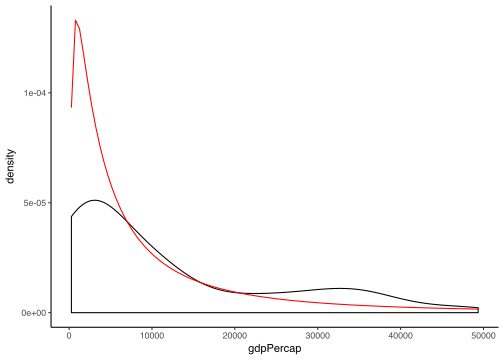
\includegraphics{17_brms_files/figure-latex/unnamed-chunk-160-1.pdf}

Näeme, et sigma hinnang on väga usaldusväärne, samas kui gruppide
vahelise sd hinnang ei ole seda mitte (pane tähele posterioorse jaotuse
ebasümmeetrilisust).

\begin{Shaded}
\begin{Highlighting}[]
\NormalTok{model2 <-}\StringTok{ }\KeywordTok{posterior_samples}\NormalTok{(m2)}
\NormalTok{pars <-}\StringTok{ }\KeywordTok{colnames}\NormalTok{(model2)}
\KeywordTok{mcmc_intervals}\NormalTok{(model2, }\DataTypeTok{regex_pars =} \StringTok{"[^(lp__)]"}\NormalTok{)}
\end{Highlighting}
\end{Shaded}

\includegraphics{17_brms_files/figure-latex/unnamed-chunk-161-1.pdf}

\begin{Shaded}
\begin{Highlighting}[]
\KeywordTok{mcmc_areas}\NormalTok{(model2,  }\DataTypeTok{pars =} \KeywordTok{c}\NormalTok{(}\StringTok{"b_Petal.Length"}\NormalTok{, }\StringTok{"b_Sepal.Width"}\NormalTok{))}
\end{Highlighting}
\end{Shaded}

\includegraphics{17_brms_files/figure-latex/unnamed-chunk-161-2.pdf}

\subsubsection{Bayesi versioon
R-ruudust}\label{bayesi-versioon-r-ruudust}

Kui suurt osa koguvarieeruvusest suudavad mudeli prediktorid seletada?

\begin{Shaded}
\begin{Highlighting}[]
\KeywordTok{bayes_R2}\NormalTok{(m2)}
\end{Highlighting}
\end{Shaded}

\begin{verbatim}
##     Estimate   Est.Error      Q2.5     Q97.5
## R2 0.8596074 0.008305745 0.8402698 0.8727995
\end{verbatim}

\begin{Shaded}
\begin{Highlighting}[]
\KeywordTok{bayes_R2}\NormalTok{(m1)}
\end{Highlighting}
\end{Shaded}

\begin{verbatim}
##     Estimate  Est.Error      Q2.5     Q97.5
## R2 0.8328977 0.01092087 0.8073688 0.8497679
\end{verbatim}

\url{https://github.com/jgabry/bayes_R2/blob/master/bayes_R2.pdf} Annab
põhjenduse sellele statistikule (mille arvutamine erineb tavalisest
vähimruutudega arvutatud mudeli \(R^2\)-st).

\subsubsection{Plotime mudeli poolt ennustatud valimeid -- posterior
predictive
check}\label{plotime-mudeli-poolt-ennustatud-valimeid-posterior-predictive-check}

Kui mudel suudab genereerida simuleeritud valimeid, mis ei erine väga
palju empiirilisest valimist, mille põhjal see mudel fititi, siis
võib-olla ei ole see täiesti ebaõnnestunud mudeldamine. See on loogika
posterioorse ennustava ploti taga.

Vaatame siin simultaanselt kõigi kolme eelnevalt fititud mudeli
simuleeritud valimeid (y\_rep) võrdluses algsete andmetega (y):

\begin{Shaded}
\begin{Highlighting}[]
\NormalTok{purrr}\OperatorTok{::}\KeywordTok{map}\NormalTok{(}\KeywordTok{list}\NormalTok{(m1, m2, m3), pp_check, }\DataTypeTok{nsamples =} \DecValTok{10}\NormalTok{) }\OperatorTok\StringTok{ }
\StringTok{  }\KeywordTok{grid.arrange}\NormalTok{(}\DataTypeTok{grobs =}\NormalTok{ ., }\DataTypeTok{nrow =} \DecValTok{3}\NormalTok{)}
\end{Highlighting}
\end{Shaded}

\includegraphics{17_brms_files/figure-latex/unnamed-chunk-164-1.pdf}

\begin{itemize}
\tightlist
\item
  y - tihedusplot empiirilistest andmetest
\item
  y\_rep -- plotid mudeli poolt ennustatud iseseisvatest valimitest
  (igaüks sama suur kui empiiriline valim y) Jooniselt on näha, et m3
  ennustused on võrreldes m1 ja m2-ga kõige kaugemal tegelikust
  valimist.
\end{itemize}

\subsubsection{Plotime mudeli ennustusi - marginal effects
plots}\label{plotime-mudeli-ennustusi---marginal-effects-plots}

Teeme ennustused. Kõigepealt ennustame ühe keskmise mudeliga, mis ei
arvesta mitmetasemelise mudeli madalamte tasemete koefitsientidega.

\begin{Shaded}
\begin{Highlighting}[]
\KeywordTok{plot}\NormalTok{(}\KeywordTok{marginal_effects}\NormalTok{(m2, }\DataTypeTok{effects =} \StringTok{"Petal.Length"}\NormalTok{, }\DataTypeTok{method =} \StringTok{"predict"}\NormalTok{, }\DataTypeTok{probs =} \KeywordTok{c}\NormalTok{(}\FloatTok{0.1}\NormalTok{, }\FloatTok{0.9}\NormalTok{)), }\DataTypeTok{points =} \OtherTok{TRUE}\NormalTok{)}
\end{Highlighting}
\end{Shaded}

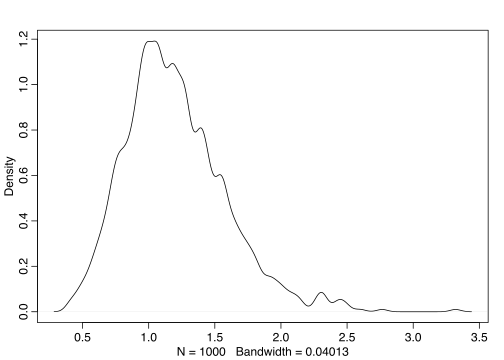
\includegraphics{17_brms_files/figure-latex/unnamed-chunk-165-1.pdf}

Ennustus on selles mõttes ok, et vaid väike osa punkte jääb sellest
välja, aga laiavõitu teine!

Nüüd ennustame sama mudeli põhjal igale liigile eraldi. Seega kasutame
mudeli madalama taseme koefitsiente. Peame andma lisaparameetri
\texttt{re\_formula\ =\ NULL}, mis tagab, et ennustuse tegemisel
kasutatakse ka mudeli madalama taseme koefitsiente.

\begin{Shaded}
\begin{Highlighting}[]
\KeywordTok{plot}\NormalTok{(}\KeywordTok{marginal_effects}\NormalTok{(m2, }\DataTypeTok{effects =} \StringTok{"Petal.Length"}\NormalTok{, }\DataTypeTok{method =} \StringTok{"predict"}\NormalTok{, }\DataTypeTok{conditions =} \KeywordTok{make_conditions}\NormalTok{(iris, }\DataTypeTok{vars =} \StringTok{"Species"}\NormalTok{), }\DataTypeTok{probs =} \KeywordTok{c}\NormalTok{(}\FloatTok{0.1}\NormalTok{, }\FloatTok{0.9}\NormalTok{), }\DataTypeTok{re_formula =} \OtherTok{NULL}\NormalTok{), }\DataTypeTok{points =} \OtherTok{TRUE}\NormalTok{)}
\end{Highlighting}
\end{Shaded}

\includegraphics{17_brms_files/figure-latex/unnamed-chunk-166-1.pdf}

\texttt{method\ =\ "predict"} ennustab, millisesse vahemikku peaks
mudeli järgi jääma 90\% andmepunkte (k.a. uued andmepunktid, mida pole
veel valimisse korjatud).

Tõesti, valdav enamus valimi punkte on intervallis sees, mis viitab et
mudel töötab hästi. Seal, kus on rohkem punkte, on intervall kitsam ja
mudel usaldusväärsem.

Järgneval pildil on \texttt{method\ =\ "fitted"}. Nüüd on enamus punkte
väljaspool usaldusintervalle, mis sellel pildil mõõdavad meie usaldust
regressioonijoone vastu.

\begin{Shaded}
\begin{Highlighting}[]
\KeywordTok{plot}\NormalTok{(}\KeywordTok{marginal_effects}\NormalTok{(m2, }\DataTypeTok{effects =} \StringTok{"Petal.Length"}\NormalTok{, }\DataTypeTok{method =} \StringTok{"fitted"}\NormalTok{, }\DataTypeTok{conditions =} \KeywordTok{make_conditions}\NormalTok{(iris, }\DataTypeTok{vars =} \StringTok{"Species"}\NormalTok{), }\DataTypeTok{probs =} \KeywordTok{c}\NormalTok{(}\FloatTok{0.1}\NormalTok{, }\FloatTok{0.9}\NormalTok{), }\DataTypeTok{re_formula =} \OtherTok{NULL}\NormalTok{), }\DataTypeTok{points =} \OtherTok{TRUE}\NormalTok{)}
\end{Highlighting}
\end{Shaded}

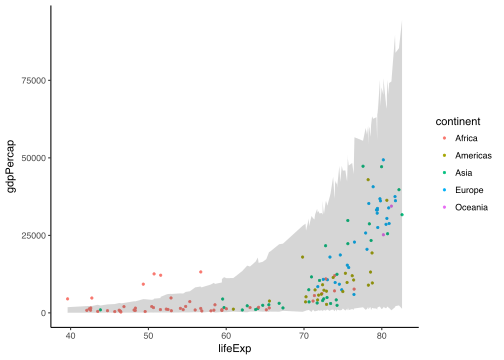
\includegraphics{17_brms_files/figure-latex/unnamed-chunk-167-1.pdf}
\texttt{method\ =\ "fitted"} annab CI regressioonijoonele.

Argumendid:

\begin{itemize}
\item
  method -- predict annab veapiirid (95\% CI) mudeli ennustustustele
  andmepunkti tasemel. fitted annab veapiirid mudeli fitile endale
  (joonele, mis tähistab keskmist või kõige tõenäolisemat y muutuja
  väärtust igal x-i väärtusel)
\item
  conditions - andmeraam, kus on kirjas mudeli nendele ennustavatele (x)
  muutujatele omistatud väärtused, mida ei joonistata x teljele. Kuna
  meil on selleks mudeli madalama taseme muutuja Species, siis on lisaks
  vaja määrata argument \emph{re\_formula = NULL}, mis tagab, et
  ennustuste tegemisel kasutatakse mudeli kõikide tasemete fititud
  koefitsiente. re\_formula = NA annab seevastu keskmise fiti üle kõigi
  gruppide (irise liikide)
\item
  probs annab usaldusintervalli piirid.
\end{itemize}

Pane tähele, et argument \texttt{points} (ja muud lisaargumendid, nagu
näiteks \texttt{theme}) kuuluvad \texttt{plot()}, mitte
\texttt{marginal\_effects()} funktsioonile.

Tavaline interaktsioonimudel, aga pidevatele muutujatele.

\begin{Shaded}
\begin{Highlighting}[]
\NormalTok{m5 <-}\StringTok{ }\KeywordTok{brm}\NormalTok{(Sepal.Length }\OperatorTok{~}\StringTok{ }\NormalTok{Petal.Length }\OperatorTok{+}\StringTok{ }\NormalTok{Sepal.Width }\OperatorTok{+}\StringTok{ }\NormalTok{Petal.Length }\OperatorTok{*}\StringTok{ }\NormalTok{Sepal.Width, }
          \DataTypeTok{data =}\NormalTok{ iris, }
          \DataTypeTok{prior =}\NormalTok{ prior, }
          \DataTypeTok{family =}\NormalTok{ gaussian)}
\KeywordTok{write_rds}\NormalTok{(m5, }\DataTypeTok{path =} \StringTok{"data/m5.fit"}\NormalTok{)}
\end{Highlighting}
\end{Shaded}

Kõigepealt plotime mudeli ennustused, kuidas Sepal Length sõltub Petal
Length-ist kolmel erineval Sepal width väärtusel.

\begin{Shaded}
\begin{Highlighting}[]
\KeywordTok{plot}\NormalTok{(}\KeywordTok{marginal_effects}\NormalTok{(m5, }\DataTypeTok{effects =} \StringTok{"Petal.Length:Sepal.Width"}\NormalTok{), }\DataTypeTok{points =} \OtherTok{TRUE}\NormalTok{)}
\end{Highlighting}
\end{Shaded}

\includegraphics{17_brms_files/figure-latex/unnamed-chunk-170-1.pdf}

Ja siis sümmeetriliselt vastupidi.

\begin{Shaded}
\begin{Highlighting}[]
\KeywordTok{plot}\NormalTok{(}\KeywordTok{marginal_effects}\NormalTok{(m5, }\DataTypeTok{effects =} \StringTok{"Sepal.Width:Petal.Length"}\NormalTok{), }\DataTypeTok{points =} \OtherTok{TRUE}\NormalTok{)}
\end{Highlighting}
\end{Shaded}

\includegraphics{17_brms_files/figure-latex/unnamed-chunk-171-1.pdf}

Siin lisame enda soovitud Sepal Width väärtused (5 ja 1.2), mis on
väljaspool seda, mida loodus pakub. Pane tähele ennustuse laiemaid CI-e.

\begin{Shaded}
\begin{Highlighting}[]
\NormalTok{conditions <-}\StringTok{ }\KeywordTok{data.frame}\NormalTok{(}\DataTypeTok{Sepal.Width =} \KeywordTok{c}\NormalTok{(}\DecValTok{5}\NormalTok{, }\FloatTok{1.2}\NormalTok{))}
\KeywordTok{plot}\NormalTok{(}\KeywordTok{marginal_effects}\NormalTok{(m5, }\DataTypeTok{effects =} \StringTok{"Petal.Length"}\NormalTok{, }\DataTypeTok{conditions =}\NormalTok{ conditions, }\DataTypeTok{re_formula =} \OtherTok{NULL}\NormalTok{), }\DataTypeTok{points =} \OtherTok{TRUE}\NormalTok{)}
\end{Highlighting}
\end{Shaded}

\includegraphics{17_brms_files/figure-latex/unnamed-chunk-172-1.pdf}

\subsubsection{Alternatiivne tee}\label{alternatiivne-tee}

Alternatiivne millele? Teeme tabeli nende väärtustega, millele tahame
mudeli ennustusi. Tabelis newx on spetsifitseeritud mudeli kõikide X
muutujate väärtused! Me ennustame Y väärtusi paljudel meie poolt võrdse
vahemaaga ette antud petal length väärtustel, kusjuures me hoiame sepal
width väärtuse alati konstantsena tema valimi keskmisel väärtusel ja
vaatame ennustusi eraldi kahele liigile kolmest. Liigid on mudeli madala
taseme osad, seega kasutame ennustuste tegemisel mudeli kõikide tasemete
koefitsiente.

\begin{Shaded}
\begin{Highlighting}[]
\NormalTok{newx <-}\StringTok{ }\KeywordTok{expand.grid}\NormalTok{(}\DataTypeTok{Petal.Length =}\NormalTok{ modelr}\OperatorTok{::}\KeywordTok{seq_range}\NormalTok{(iris}\OperatorTok{$}\NormalTok{Petal.Length, }\DataTypeTok{n =} \DecValTok{150}\NormalTok{),}
                    \DataTypeTok{Sepal.Width =} \KeywordTok{mean}\NormalTok{(iris}\OperatorTok{$}\NormalTok{Sepal.Width),}
                    \DataTypeTok{Species =} \KeywordTok{c}\NormalTok{(}\StringTok{"setosa"}\NormalTok{, }\StringTok{"virginica"}\NormalTok{))}
\end{Highlighting}
\end{Shaded}

\texttt{expand.grid()} lõõb tabeli pikaks nii, et kõik võimalikud
kombinatsioonid 3st muutujast on täidetud väärtustega.

\texttt{re\_formula} NULL mudeldab eraldi liigid eraldi mudeli madalama
taseme (liikide sees) koefitsiente kasutades

\begin{Shaded}
\begin{Highlighting}[]
\NormalTok{predict_interval_brms2 <-}\StringTok{ }\KeywordTok{predict}\NormalTok{(m2, }\DataTypeTok{newdata =}\NormalTok{ newx, }\DataTypeTok{re_formula =} \OtherTok{NULL}\NormalTok{) }\OperatorTok
\StringTok{  }\KeywordTok{cbind}\NormalTok{(newx, .)}
\KeywordTok{head}\NormalTok{(predict_interval_brms2)}
\end{Highlighting}
\end{Shaded}

\begin{verbatim}
##   Petal.Length Sepal.Width Species Estimate Est.Error     Q2.5    Q97.5
## 1     1.000000    3.057333  setosa 4.495043 0.3228168 3.834202 5.122569
## 2     1.039597    3.057333  setosa 4.510119 0.3172937 3.879872 5.134090
## 3     1.079195    3.057333  setosa 4.543164 0.3090262 3.944452 5.163923
## 4     1.118792    3.057333  setosa 4.579237 0.3224834 3.967241 5.214037
## 5     1.158389    3.057333  setosa 4.609515 0.3210450 3.975439 5.253325
## 6     1.197987    3.057333  setosa 4.635733 0.3204683 3.978648 5.255431
\end{verbatim}

\texttt{predict()} ennustab uusi petal length väärtusi (Estimate veerg)
koos usaldusinetrvalliga neile väärtustele

Siin siis eraldi ennustused kahele liigile kolmest, kaasa arvatud petal
length väärtusvahemikule, kus selle liigi isendeid valimis ei ole (ja
võib-olla ei saagi olla)

\begin{Shaded}
\begin{Highlighting}[]
\NormalTok{no_versicolor <-}\StringTok{ }\KeywordTok{filter}\NormalTok{(iris, Species }\OperatorTok{!=}\StringTok{ "versicolor"}\NormalTok{)}
\KeywordTok{ggplot}\NormalTok{(}\DataTypeTok{data =}\NormalTok{ predict_interval_brms2, }\KeywordTok{aes}\NormalTok{(}\DataTypeTok{x =}\NormalTok{ Petal.Length, }\DataTypeTok{y =}\NormalTok{ Estimate)) }\OperatorTok{+}
\StringTok{  }\KeywordTok{geom_point}\NormalTok{(}\DataTypeTok{data =}\NormalTok{ no_versicolor, }\KeywordTok{aes}\NormalTok{(Petal.Length, Sepal.Length, }\DataTypeTok{color =}\NormalTok{ Species)) }\OperatorTok{+}
\StringTok{  }\KeywordTok{geom_line}\NormalTok{(}\KeywordTok{aes}\NormalTok{(}\DataTypeTok{color =}\NormalTok{ Species)) }\OperatorTok{+}
\StringTok{  }\KeywordTok{geom_ribbon}\NormalTok{(}\KeywordTok{aes}\NormalTok{(}\DataTypeTok{ymin =}\NormalTok{ Q2.}\DecValTok{5}\NormalTok{, }\DataTypeTok{ymax =}\NormalTok{ Q97.}\DecValTok{5}\NormalTok{, }\DataTypeTok{fill =}\NormalTok{ Species), }\DataTypeTok{alpha =} \DecValTok{1}\OperatorTok{/}\DecValTok{3}\NormalTok{)}
\end{Highlighting}
\end{Shaded}

\includegraphics{17_brms_files/figure-latex/unnamed-chunk-175-1.pdf}

Ennustav plot - kuidas lähevad kokku mudeli ennustused reaalsete y-i
andmepunktidega

\begin{Shaded}
\begin{Highlighting}[]
\NormalTok{pr <-}\StringTok{ }\KeywordTok{predict}\NormalTok{(m2) }\OperatorTok\StringTok{ }\KeywordTok{cbind}\NormalTok{(iris)}
\KeywordTok{ggplot}\NormalTok{(pr, }\KeywordTok{aes}\NormalTok{(Sepal.Length, Estimate, }\DataTypeTok{color =}\NormalTok{ Species)) }\OperatorTok{+}
\StringTok{  }\KeywordTok{geom_pointrange}\NormalTok{(}\KeywordTok{aes}\NormalTok{(}\DataTypeTok{ymin =}\NormalTok{ Q2.}\DecValTok{5}\NormalTok{, }\DataTypeTok{ymax =}\NormalTok{ Q97.}\DecValTok{5}\NormalTok{)) }\OperatorTok{+}
\StringTok{  }\KeywordTok{geom_abline}\NormalTok{(}\DataTypeTok{lty =} \DecValTok{2}\NormalTok{) }\OperatorTok{+}
\StringTok{  }\KeywordTok{coord_cartesian}\NormalTok{(}\DataTypeTok{xlim =} \KeywordTok{c}\NormalTok{(}\DecValTok{4}\NormalTok{, }\DecValTok{8}\NormalTok{), }\DataTypeTok{ylim =} \KeywordTok{c}\NormalTok{(}\DecValTok{4}\NormalTok{, }\DecValTok{8}\NormalTok{))}
\end{Highlighting}
\end{Shaded}

\includegraphics{17_brms_files/figure-latex/unnamed-chunk-176-1.pdf}

Igale andmepunktile -- kui palju erineb selle residuaal 0-st kui hästi
ennustab mudel just seda andmepunkti. Ruumi kokkuhoiuks plotime välja
ainult irise valiku 50-st andmepunktist.

\begin{Shaded}
\begin{Highlighting}[]
\KeywordTok{set.seed}\NormalTok{(}\DecValTok{69}\NormalTok{)}
\KeywordTok{as_data_frame}\NormalTok{(}\KeywordTok{residuals}\NormalTok{(m2)) }\OperatorTok\StringTok{ }
\StringTok{  }\KeywordTok{sample_n}\NormalTok{(}\DecValTok{50}\NormalTok{) }\OperatorTok\StringTok{ }
\StringTok{  }\KeywordTok{ggplot}\NormalTok{(}\KeywordTok{aes}\NormalTok{(}\DataTypeTok{x =} \KeywordTok{reorder}\NormalTok{(}\KeywordTok{seq_along}\NormalTok{(Estimate), Estimate), }\DataTypeTok{y =}\NormalTok{ Estimate)) }\OperatorTok{+}
\StringTok{  }\KeywordTok{geom_pointrange}\NormalTok{(}\KeywordTok{aes}\NormalTok{(}\DataTypeTok{ymin =}\NormalTok{ Q2.}\DecValTok{5}\NormalTok{, }\DataTypeTok{ymax =}\NormalTok{ Q97.}\DecValTok{5}\NormalTok{), }\DataTypeTok{fatten =} \FloatTok{0.1}\NormalTok{) }\OperatorTok{+}
\StringTok{  }\KeywordTok{coord_flip}\NormalTok{() }\OperatorTok{+}
\StringTok{  }\KeywordTok{theme}\NormalTok{(}\DataTypeTok{text =} \KeywordTok{element_text}\NormalTok{(}\DataTypeTok{size =} \DecValTok{8}\NormalTok{), }\DataTypeTok{axis.title.y =} \KeywordTok{element_blank}\NormalTok{()) }\OperatorTok{+}
\StringTok{  }\KeywordTok{xlab}\NormalTok{(}\StringTok{"Residuals (95 CI)"}\NormalTok{)}
\end{Highlighting}
\end{Shaded}

\includegraphics{17_brms_files/figure-latex/unnamed-chunk-177-1.pdf}

Ok, isendid nr 15 ja 44 paistavad olema vastavalt palju suurema ja
väiksema Sepal Lengthiga kui mudel ennustab. Võib küsida, miks?

Nüüd plotime usaldusintervalli mudeli fitile (`keskmisele' Y väärtusele
igal määratud X-i väärtusel), mitte Y-ennustusele andmepunkti kaupa.
Selleks on hea fitted() funktsioon. Me ennustame m2 mudelist vastavalt
newdata parameetriväärtustele. Kui me newdata argumendi tühjaks jätame,
siis võtab fitted() selleks automaatselt algse iris tabeli (ehk valimi
väärtused).

\begin{Shaded}
\begin{Highlighting}[]
\NormalTok{predict_interval_brms2f <-}\StringTok{ }\KeywordTok{fitted}\NormalTok{(m2, }\DataTypeTok{newdata =}\NormalTok{ newx, }\DataTypeTok{re_formula =} \OtherTok{NULL}\NormalTok{) }\OperatorTok
\StringTok{  }\KeywordTok{cbind}\NormalTok{(newx,.)}
\KeywordTok{head}\NormalTok{(predict_interval_brms2f)}
\end{Highlighting}
\end{Shaded}

\begin{verbatim}
##   Petal.Length Sepal.Width Species Estimate  Est.Error     Q2.5    Q97.5
## 1     1.000000    3.057333  setosa 4.490401 0.05417915 4.382898 4.593559
## 2     1.039597    3.057333  setosa 4.520443 0.05347147 4.414865 4.622773
## 3     1.079195    3.057333  setosa 4.550485 0.05287770 4.445885 4.652773
## 4     1.118792    3.057333  setosa 4.580528 0.05240171 4.477761 4.682077
## 5     1.158389    3.057333  setosa 4.610570 0.05204672 4.508861 4.711120
## 6     1.197987    3.057333  setosa 4.640612 0.05181523 4.539425 4.741384
\end{verbatim}

\begin{Shaded}
\begin{Highlighting}[]
\KeywordTok{ggplot}\NormalTok{(}\DataTypeTok{data =}\NormalTok{ predict_interval_brms2f, }\KeywordTok{aes}\NormalTok{(}\DataTypeTok{x =}\NormalTok{ Petal.Length, }\DataTypeTok{y =}\NormalTok{ Estimate, }\DataTypeTok{color =}\NormalTok{ Species)) }\OperatorTok{+}
\StringTok{  }\KeywordTok{geom_point}\NormalTok{(}\DataTypeTok{data =}\NormalTok{ no_versicolor, }\KeywordTok{aes}\NormalTok{(Petal.Length, Sepal.Length, }\DataTypeTok{color =}\NormalTok{ Species)) }\OperatorTok{+}
\StringTok{  }\KeywordTok{geom_line}\NormalTok{() }\OperatorTok{+}
\StringTok{  }\KeywordTok{geom_ribbon}\NormalTok{(}\KeywordTok{aes}\NormalTok{(}\DataTypeTok{ymin =}\NormalTok{ Q2.}\DecValTok{5}\NormalTok{, }\DataTypeTok{ymax =}\NormalTok{ Q97.}\DecValTok{5}\NormalTok{, }\DataTypeTok{fill =}\NormalTok{ Species), }\DataTypeTok{alpha =} \DecValTok{1}\OperatorTok{/}\DecValTok{3}\NormalTok{, }\DataTypeTok{colour =} \OtherTok{NA}\NormalTok{) }\OperatorTok{+}
\StringTok{  }\KeywordTok{scale_x_continuous}\NormalTok{(}\DataTypeTok{breaks =} \DecValTok{0}\OperatorTok{:}\DecValTok{10}\NormalTok{)}
\end{Highlighting}
\end{Shaded}

\includegraphics{17_brms_files/figure-latex/unnamed-chunk-179-1.pdf}

Mudeli genereeritud andmed ja valimiandmed mõõtmisobjekti (subjekti e
taimeisendi) kaupa. See on sisuliselt posterior predictive plot (vt
eespool).

\begin{Shaded}
\begin{Highlighting}[]
\NormalTok{predicted_subjects_brms <-}\StringTok{ }\KeywordTok{predict}\NormalTok{(m2) }\OperatorTok\StringTok{ }\KeywordTok{cbind}\NormalTok{(iris, .)}
\end{Highlighting}
\end{Shaded}

\texttt{predict()} arvutab mudeli põhjal uusi Y muutuja andmepunkte.
Võib kasutada ka väljamõeldud andmete pealt Y väärtuste ennustamiseks
(selleks tuleb anda ette andmeraam kõigi X-muutujate väärtustega, mille
pealt tahetakse ennustusi).

Punktid on ennustused ja ristikesed on valimiandmed

\begin{Shaded}
\begin{Highlighting}[]
\KeywordTok{ggplot}\NormalTok{(}\DataTypeTok{data =}\NormalTok{ predicted_subjects_brms, }\KeywordTok{aes}\NormalTok{(}\DataTypeTok{x =}\NormalTok{ Petal.Length, }\DataTypeTok{color =}\NormalTok{ Species)) }\OperatorTok{+}
\StringTok{  }\KeywordTok{geom_point}\NormalTok{(}\KeywordTok{aes}\NormalTok{(}\DataTypeTok{y =}\NormalTok{ Estimate)) }\OperatorTok{+}
\StringTok{  }\KeywordTok{geom_point}\NormalTok{(}\KeywordTok{aes}\NormalTok{(}\DataTypeTok{y =}\NormalTok{ Sepal.Length), }\DataTypeTok{shape =} \DecValTok{3}\NormalTok{)}
\end{Highlighting}
\end{Shaded}

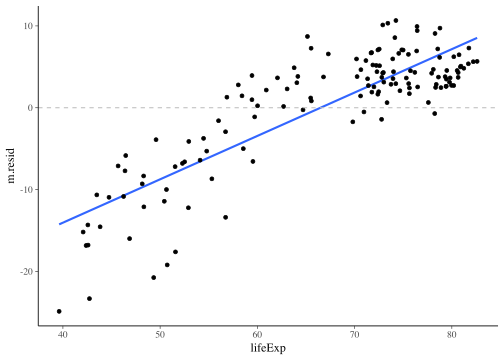
\includegraphics{17_brms_files/figure-latex/unnamed-chunk-181-1.pdf}

\subsubsection{Alternatiiv --
ansambliennustus}\label{alternatiiv-ansambliennustus}

Kuna meil on 2 mudelit (m2 ja m3) mis on pea võrdselt eelistatud, siis
genreerime ennustused mõlemast (mudelite ansamblist) proportsionaalselt
nende waic skooridega. See ennustus kajastab meie mudeldamistööd
tervikuna, mitte ühte ``parimat'' mudelit ja seega võib loota, et annab
paremini edasi meie mudeldamises peituvat ebakindlust.

\begin{Shaded}
\begin{Highlighting}[]
\NormalTok{pp_a <-}\StringTok{ }\KeywordTok{pp_average}\NormalTok{(m2, m3, }\DataTypeTok{weights =} \StringTok{"waic"}\NormalTok{, }\DataTypeTok{method =} \StringTok{"predict"}\NormalTok{) }\OperatorTok
\StringTok{  }\KeywordTok{as_tibble}\NormalTok{() }\OperatorTok\StringTok{ }
\StringTok{  }\KeywordTok{bind_cols}\NormalTok{(iris)}
\KeywordTok{ggplot}\NormalTok{(}\DataTypeTok{data =}\NormalTok{ pp_a, }\KeywordTok{aes}\NormalTok{(}\DataTypeTok{x =}\NormalTok{ Petal.Length, }\DataTypeTok{color =}\NormalTok{ Species)) }\OperatorTok{+}
\StringTok{  }\KeywordTok{geom_point}\NormalTok{(}\KeywordTok{aes}\NormalTok{(}\DataTypeTok{y =}\NormalTok{ Estimate)) }\OperatorTok{+}
\StringTok{  }\KeywordTok{geom_point}\NormalTok{(}\KeywordTok{aes}\NormalTok{(}\DataTypeTok{y =}\NormalTok{ Sepal.Length), }\DataTypeTok{shape =} \DecValTok{3}\NormalTok{)}
\end{Highlighting}
\end{Shaded}

\subsection{Mudeli eelduste kontroll}\label{mudeli-eelduste-kontroll}

Pareto k otsib nn mõjukaid (influential) andmepunkte.

\begin{Shaded}
\begin{Highlighting}[]
\NormalTok{loo_m2 <-}\StringTok{ }\KeywordTok{loo}\NormalTok{(m2)}
\KeywordTok{plot}\NormalTok{(loo_m2)}
\end{Highlighting}
\end{Shaded}

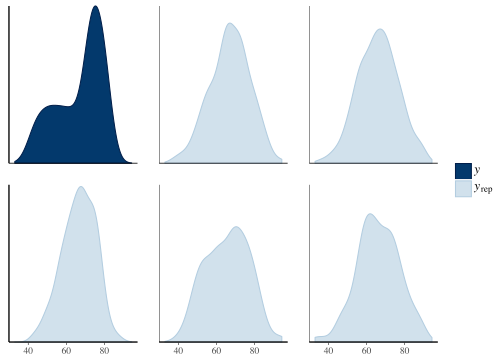
\includegraphics{17_brms_files/figure-latex/unnamed-chunk-183-1.pdf}

Kui paljud andmepunktid on kahtlaselt mõjukad?

\begin{Shaded}
\begin{Highlighting}[]
\KeywordTok{pareto_k_table}\NormalTok{(loo_m2) }
\end{Highlighting}
\end{Shaded}

\begin{verbatim}
## 
## All Pareto k estimates are good (k < 0.5).
\end{verbatim}

\subsubsection{Plotime residuaalid}\label{plotime-residuaalid}

\texttt{resid()} annab residuaalid vektorina. Kõigepealt plotime
residuaalid fititud (keskmiste) Y väärtuste vastu:

\begin{Shaded}
\begin{Highlighting}[]
\NormalTok{resid <-}\StringTok{ }\KeywordTok{residuals}\NormalTok{(m2, }\DataTypeTok{type =} \StringTok{"pearson"}\NormalTok{)}
\NormalTok{fit <-}\StringTok{ }\KeywordTok{fitted}\NormalTok{(m2)}
\KeywordTok{ggplot}\NormalTok{() }\OperatorTok{+}\StringTok{ }
\StringTok{  }\KeywordTok{geom_point}\NormalTok{(}\KeywordTok{aes}\NormalTok{(}\DataTypeTok{x =}\NormalTok{ fit[,}\StringTok{"Estimate"}\NormalTok{], }\DataTypeTok{y =}\NormalTok{ resid[,}\StringTok{"Estimate"}\NormalTok{])) }\OperatorTok{+}\StringTok{ }
\StringTok{  }\KeywordTok{geom_hline}\NormalTok{(}\DataTypeTok{yintercept =} \DecValTok{0}\NormalTok{, }\DataTypeTok{lty =} \StringTok{"dashed"}\NormalTok{) }\OperatorTok{+}
\StringTok{  }\KeywordTok{labs}\NormalTok{(}\DataTypeTok{x =} \StringTok{"fitted"}\NormalTok{, }\DataTypeTok{y =} \StringTok{"residuals"}\NormalTok{)}
\end{Highlighting}
\end{Shaded}

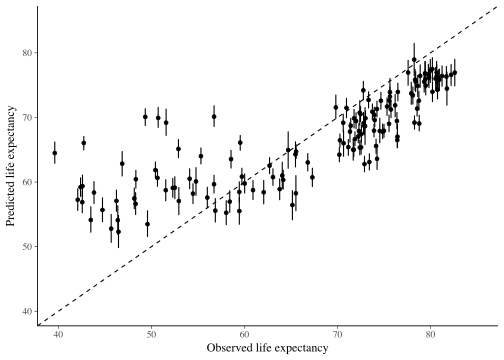
\includegraphics{17_brms_files/figure-latex/unnamed-chunk-185-1.pdf}

Residuals vs fitted plot testib lineaarsuse eeldust - kui .resid punktid
jaotuvad ühtlaselt nulli ümber, siis mudel püüab kinni kogu
süstemaatilise varieeruvuse teie andmetest ja see mis üle jääb on
juhuslik varieeruvus.

Vaatame diagnostilist plotti autokorrelatsioonist residuaalide vahel.

\begin{Shaded}
\begin{Highlighting}[]
\KeywordTok{plot}\NormalTok{(}\KeywordTok{acf}\NormalTok{(resid))}
\end{Highlighting}
\end{Shaded}

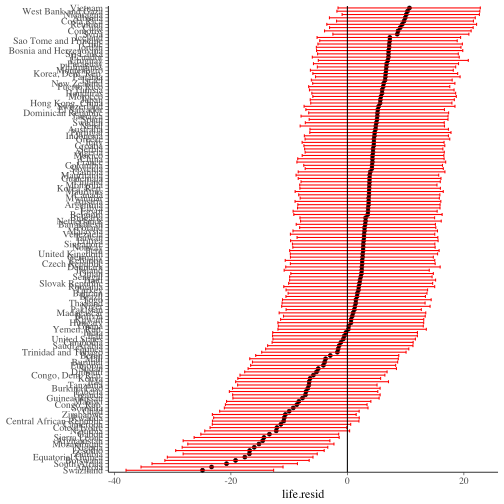
\includegraphics{17_brms_files/figure-latex/unnamed-chunk-186-1.pdf}
\includegraphics{17_brms_files/figure-latex/unnamed-chunk-186-2.pdf}

Residuaalide autokorrelatsioonid on madalad - seega kõik paistab OK ja
andmepunktide sõltumatus on tagatud.

Siin on residuaalide histogramm:

\begin{Shaded}
\begin{Highlighting}[]
\KeywordTok{ggplot}\NormalTok{(}\DataTypeTok{data =} \OtherTok{NULL}\NormalTok{) }\OperatorTok{+}\StringTok{ }
\StringTok{  }\KeywordTok{geom_density}\NormalTok{(}\KeywordTok{aes}\NormalTok{(}\DataTypeTok{x =}\NormalTok{ resid[,}\StringTok{"Estimate"}\NormalTok{]), }\DataTypeTok{fill =} \StringTok{"lightgrey"}\NormalTok{) }\OperatorTok{+}\StringTok{ }
\StringTok{  }\KeywordTok{geom_vline}\NormalTok{(}\DataTypeTok{xintercept =} \KeywordTok{median}\NormalTok{(resid), }\DataTypeTok{linetype =} \StringTok{"dashed"}\NormalTok{)}
\end{Highlighting}
\end{Shaded}

\includegraphics{17_brms_files/figure-latex/unnamed-chunk-187-1.pdf}

Residuaalid on sümmeetrilise jaotusega ja meedian residuaal on peaaegu
null. See on kõik hea.

Ja lõpuks plotime residuaalid kõigi x-muutujate vastu. Kõigepealt
ühendame resid vektori irise tabeliga, et oleks mugavam plottida,
seejärel tekitame uue veeru st\_resid e studentiseeritud residuaalid,
mis on sd ühikutes.

residuaalid standardhälbe ühikutes (nn Studentiseeritud residuaalid)
saab ja ka tuleks plottida kõigi x-muutujate suhtes.

\begin{Shaded}
\begin{Highlighting}[]
\NormalTok{iris2 <-}\StringTok{ }\NormalTok{iris }\OperatorTok\StringTok{ }
\StringTok{  }\KeywordTok{cbind}\NormalTok{(resid) }\OperatorTok\StringTok{ }
\StringTok{  }\KeywordTok{mutate}\NormalTok{(}\DataTypeTok{st_resid =}\NormalTok{ Estimate }\OperatorTok{/}\StringTok{ }\KeywordTok{sd}\NormalTok{(resid))}
\KeywordTok{ggplot}\NormalTok{(iris2, }\KeywordTok{aes}\NormalTok{(Petal.Length, st_resid, }\DataTypeTok{color =}\NormalTok{ Species)) }\OperatorTok{+}\StringTok{ }
\StringTok{  }\KeywordTok{geom_point}\NormalTok{() }\OperatorTok{+}
\StringTok{  }\KeywordTok{geom_hline}\NormalTok{(}\DataTypeTok{yintercept =} \DecValTok{0}\NormalTok{, }\DataTypeTok{linetype =} \StringTok{"dashed"}\NormalTok{)}
\end{Highlighting}
\end{Shaded}

\includegraphics{17_brms_files/figure-latex/unnamed-chunk-188-1.pdf}

Tsiteerides klassikuid: ``Pole paha!''. Mudel ennustab hästi, aga mõne
punkti jaoks on ennustus 2 sd kaugusel.

\begin{Shaded}
\begin{Highlighting}[]
\KeywordTok{ggplot}\NormalTok{(iris2, }\KeywordTok{aes}\NormalTok{(Sepal.Width, st_resid, }\DataTypeTok{color =}\NormalTok{ Species)) }\OperatorTok{+}\StringTok{ }
\StringTok{  }\KeywordTok{geom_point}\NormalTok{() }\OperatorTok{+}
\StringTok{  }\KeywordTok{geom_hline}\NormalTok{(}\DataTypeTok{yintercept =} \DecValTok{0}\NormalTok{, }\DataTypeTok{linetype =} \StringTok{"dashed"}\NormalTok{)}
\end{Highlighting}
\end{Shaded}

\includegraphics{17_brms_files/figure-latex/unnamed-chunk-189-1.pdf}

\begin{Shaded}
\begin{Highlighting}[]
\KeywordTok{ggplot}\NormalTok{(iris2, }\KeywordTok{aes}\NormalTok{(Species, st_resid)) }\OperatorTok{+}\StringTok{ }
\StringTok{  }\KeywordTok{geom_boxplot}\NormalTok{() }\OperatorTok{+}
\StringTok{  }\KeywordTok{geom_hline}\NormalTok{(}\DataTypeTok{yintercept =} \DecValTok{0}\NormalTok{, }\DataTypeTok{linetype =} \StringTok{"dashed"}\NormalTok{) }\OperatorTok{+}
\StringTok{  }\KeywordTok{geom_jitter}\NormalTok{(}\DataTypeTok{width =} \FloatTok{0.1}\NormalTok{)}
\end{Highlighting}
\end{Shaded}

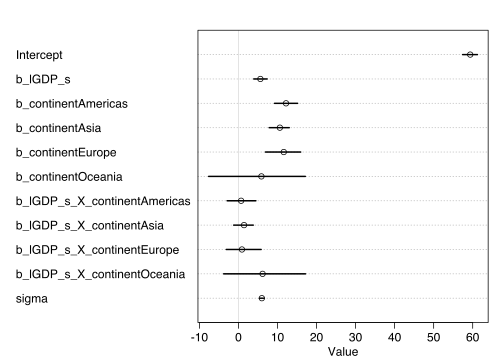
\includegraphics{17_brms_files/figure-latex/unnamed-chunk-190-1.pdf}

\section{Brms mudelid}\label{brms-mudelid}

\subsection{Robustne lineaarne
regressioon}\label{robustne-lineaarne-regressioon}

Kasutame dnorm likelihoodi asemel studenti t jaotust. Selle jaotuse õlad
on reguleeritavalt kõrgemad ja nende alla mahuvad paremini outlierid.
Õlgade kõrgust reguleerib parameeter nu (1 - Inf), mille väiksemad
väärtused (alla 10) annavad laiad õlad ja kaitse outlierite vastu. Me
anname nu-le gamma priori. Sellel prioril on omakorda 2 parameetrit,
shape ja scale Kui fikseerime shape = 4 ja scale = 1, siis saame kitsa
priori, mis eelistab nu väärtusi, mis soosivad laiu õlgu ja robustset
regressiooni.

\begin{Shaded}
\begin{Highlighting}[]
\NormalTok{x =}\StringTok{ }\KeywordTok{seq}\NormalTok{(}\DataTypeTok{from =} \DecValTok{0}\NormalTok{, }\DataTypeTok{to =} \DecValTok{20}\NormalTok{, }\DataTypeTok{by =}\NormalTok{ .}\DecValTok{1}\NormalTok{)}
\NormalTok{y =}\StringTok{ }\KeywordTok{dgamma}\NormalTok{(x, }\DataTypeTok{shape =} \DecValTok{4}\NormalTok{, }\DataTypeTok{scale =} \DecValTok{1}\NormalTok{)}
\KeywordTok{plot}\NormalTok{(y }\OperatorTok{~}\StringTok{ }\NormalTok{x)}
\end{Highlighting}
\end{Shaded}

\includegraphics{17_brms_files/figure-latex/unnamed-chunk-191-1.pdf}

\begin{Shaded}
\begin{Highlighting}[]
\KeywordTok{get_prior}\NormalTok{(Sepal.Length }\OperatorTok{~}\StringTok{ }\NormalTok{Petal.Length, }\DataTypeTok{data =}\NormalTok{ iris, }\DataTypeTok{family =} \StringTok{"student"}\NormalTok{)}
\end{Highlighting}
\end{Shaded}

\begin{verbatim}
##                 prior     class         coef group resp dpar nlpar bound
## 1                             b                                         
## 2                             b Petal.Length                            
## 3 student_t(3, 6, 10) Intercept                                         
## 4       gamma(2, 0.1)        nu                                         
## 5 student_t(3, 0, 10)     sigma
\end{verbatim}

\begin{Shaded}
\begin{Highlighting}[]
\NormalTok{prior <-}\StringTok{ }\KeywordTok{prior}\NormalTok{(}\KeywordTok{gamma}\NormalTok{(}\DecValTok{4}\NormalTok{, }\DecValTok{1}\NormalTok{), }\DataTypeTok{class =} \StringTok{"nu"}\NormalTok{)}
\end{Highlighting}
\end{Shaded}

robust\_m1 on studenti likelihoodiga, mille õlad määratakse adaptiivselt
andmete poolt. robust\_m2-s anname õlgade laiuse ette ja robust\_m3 on
mitte-robustne kontroll tavalise normaalse likelihoodiga.

\begin{Shaded}
\begin{Highlighting}[]
\NormalTok{robust_m1 <-}\StringTok{ }\KeywordTok{brm}\NormalTok{(Sepal.Length }\OperatorTok{~}\StringTok{ }\NormalTok{Petal.Length, }
          \DataTypeTok{data =}\NormalTok{ iris, }
          \DataTypeTok{family =} \StringTok{"student"}\NormalTok{,}
          \DataTypeTok{prior =}\NormalTok{ prior)}
\NormalTok{robust_m2 <-}\StringTok{ }\KeywordTok{brm}\NormalTok{(}\KeywordTok{bf}\NormalTok{(Sepal.Length}\OperatorTok{~}\NormalTok{Petal.Length, }\DataTypeTok{nu =} \DecValTok{4}\NormalTok{),}
          \DataTypeTok{data =}\NormalTok{ iris, }
          \DataTypeTok{family =}\NormalTok{ student,}
          \DataTypeTok{prior =} \KeywordTok{c}\NormalTok{(}\KeywordTok{prior}\NormalTok{(}\KeywordTok{normal}\NormalTok{(}\DecValTok{0}\NormalTok{, }\DecValTok{100}\NormalTok{), }\DataTypeTok{class =}\NormalTok{ Intercept),}
                \KeywordTok{prior}\NormalTok{(}\KeywordTok{normal}\NormalTok{(}\DecValTok{0}\NormalTok{, }\DecValTok{10}\NormalTok{),  }\DataTypeTok{class =}\NormalTok{ b),}
                \KeywordTok{prior}\NormalTok{(}\KeywordTok{student_t}\NormalTok{(}\DecValTok{5}\NormalTok{, }\DecValTok{0}\NormalTok{, }\DecValTok{5}\NormalTok{),   }\DataTypeTok{class =}\NormalTok{ sigma)))}
\NormalTok{robust_m3 <-}\StringTok{ }\KeywordTok{brm}\NormalTok{(Sepal.Length}\OperatorTok{~}\NormalTok{Petal.Length, }
          \DataTypeTok{data =}\NormalTok{ iris, }
          \DataTypeTok{family =} \StringTok{"gaussian"}\NormalTok{)}
\KeywordTok{write_rds}\NormalTok{(robust_m1, }\DataTypeTok{path =} \StringTok{"data/robust_m1.fit"}\NormalTok{)}
\KeywordTok{write_rds}\NormalTok{(robust_m2, }\DataTypeTok{path =} \StringTok{"data/robust_m2.fit"}\NormalTok{)}
\KeywordTok{write_rds}\NormalTok{(robust_m3, }\DataTypeTok{path =} \StringTok{"data/robust_m3.fit"}\NormalTok{)}
\end{Highlighting}
\end{Shaded}

\begin{Shaded}
\begin{Highlighting}[]
\NormalTok{b_estimates <-}\StringTok{ }\KeywordTok{bind_rows}\NormalTok{(}\KeywordTok{tidy}\NormalTok{(robust_m1), }
                         \KeywordTok{tidy}\NormalTok{(robust_m2), }
                         \KeywordTok{tidy}\NormalTok{(robust_m3), }
                         \DataTypeTok{.id =} \StringTok{"model_nr"}\NormalTok{) }
\NormalTok{b1 <-}\StringTok{ }\KeywordTok{filter}\NormalTok{(b_estimates, }\KeywordTok{str_detect}\NormalTok{(term, }\StringTok{"b_P"}\NormalTok{)) }\OperatorTok
\StringTok{  }\KeywordTok{ggplot}\NormalTok{(}\KeywordTok{aes}\NormalTok{(model_nr, estimate)) }\OperatorTok{+}
\StringTok{  }\KeywordTok{geom_pointrange}\NormalTok{(}\KeywordTok{aes}\NormalTok{(}\DataTypeTok{ymin =}\NormalTok{ lower, }\DataTypeTok{ymax =}\NormalTok{ upper)) }\OperatorTok{+}\StringTok{ }
\StringTok{  }\KeywordTok{coord_flip}\NormalTok{() }\OperatorTok{+}\StringTok{ }
\StringTok{  }\KeywordTok{labs}\NormalTok{(}\DataTypeTok{x =} \StringTok{"Model nr"}\NormalTok{, }\DataTypeTok{title =} \StringTok{"slopes"}\NormalTok{)}
\NormalTok{b2 <-}\StringTok{ }\KeywordTok{filter}\NormalTok{(b_estimates, }\KeywordTok{str_detect}\NormalTok{(term, }\StringTok{"b_I"}\NormalTok{)) }\OperatorTok
\StringTok{  }\KeywordTok{ggplot}\NormalTok{(}\KeywordTok{aes}\NormalTok{(model_nr, estimate)) }\OperatorTok{+}
\StringTok{  }\KeywordTok{geom_pointrange}\NormalTok{(}\KeywordTok{aes}\NormalTok{(}\DataTypeTok{ymin =}\NormalTok{ lower, }\DataTypeTok{ymax =}\NormalTok{ upper)) }\OperatorTok{+}\StringTok{ }
\StringTok{  }\KeywordTok{coord_flip}\NormalTok{() }\OperatorTok{+}\StringTok{ }
\StringTok{  }\KeywordTok{labs}\NormalTok{(}\DataTypeTok{x =} \OtherTok{NULL}\NormalTok{, }\DataTypeTok{title =} \StringTok{"intercepts"}\NormalTok{)}
\NormalTok{gridExtra}\OperatorTok{::}\KeywordTok{grid.arrange}\NormalTok{(b1, b2, }\DataTypeTok{nrow =} \DecValTok{1}\NormalTok{)}
\end{Highlighting}
\end{Shaded}

\includegraphics{17_brms_files/figure-latex/unnamed-chunk-196-1.pdf}

Kolme mudeli lõikepunktid ja tõusunurgad on sisuliselt võrdsed ja sama
täpsusega hinnatud. Seega ei tee robustne mudel vähemal halba, kui meil
on enam-vähem normaalsed andmed.

Proovime ka robuststet versiooni 2 grupi võrdlusest (vastab t testile,
kus kahe grupi sd-d hinnatakse eraldi)

\begin{Shaded}
\begin{Highlighting}[]
\NormalTok{no_versicolor <-}\StringTok{ }\KeywordTok{filter}\NormalTok{(iris, Species }\OperatorTok{!=}\StringTok{ "versicolor"}\NormalTok{)}
\KeywordTok{get_prior}\NormalTok{(}\KeywordTok{bf}\NormalTok{(Sepal.Length }\OperatorTok{~}\StringTok{ }\NormalTok{Species, sigma }\OperatorTok{~}\StringTok{ }\NormalTok{Species), }
          \DataTypeTok{data =}\NormalTok{ no_versicolor, }
          \DataTypeTok{family =} \StringTok{"student"}\NormalTok{)}
\end{Highlighting}
\end{Shaded}

\begin{verbatim}
##                 prior     class             coef group resp  dpar nlpar
## 1                             b                                        
## 2                             b Speciesvirginica                       
## 3 student_t(3, 6, 10) Intercept                                        
## 4       gamma(2, 0.1)        nu                                        
## 5                             b                             sigma      
## 6                             b Speciesvirginica            sigma      
## 7 student_t(3, 0, 10) Intercept                             sigma      
##   bound
## 1      
## 2      
## 3      
## 4      
## 5      
## 6      
## 7
\end{verbatim}

\begin{Shaded}
\begin{Highlighting}[]
\NormalTok{prior <-}\StringTok{ }\KeywordTok{c}\NormalTok{(}\KeywordTok{prior}\NormalTok{(}\KeywordTok{gamma}\NormalTok{(}\DecValTok{4}\NormalTok{, }\DecValTok{1}\NormalTok{), }\DataTypeTok{class =} \StringTok{"nu"}\NormalTok{),}
           \KeywordTok{prior}\NormalTok{(}\KeywordTok{normal}\NormalTok{(}\DecValTok{0}\NormalTok{, }\DecValTok{4}\NormalTok{), }\DataTypeTok{class =} \StringTok{"b"}\NormalTok{))}
\end{Highlighting}
\end{Shaded}

\begin{Shaded}
\begin{Highlighting}[]
\NormalTok{robust_t_test1 <-}\StringTok{ }\KeywordTok{brm}\NormalTok{(}\KeywordTok{bf}\NormalTok{(Sepal.Length }\OperatorTok{~}\StringTok{ }\NormalTok{Species, sigma }\OperatorTok{~}\StringTok{ }\NormalTok{Species), }
            \DataTypeTok{data =}\NormalTok{ no_versicolor, }
            \DataTypeTok{prior =}\NormalTok{ prior, }
            \DataTypeTok{family =} \StringTok{"student"}\NormalTok{)}
\KeywordTok{write_rds}\NormalTok{(robust_t_test1, }\DataTypeTok{path =} \StringTok{"data/robust_t_test1.fit"}\NormalTok{)}
\end{Highlighting}
\end{Shaded}

\begin{Shaded}
\begin{Highlighting}[]
\KeywordTok{tidy}\NormalTok{(robust_t_test1)}
\end{Highlighting}
\end{Shaded}

\begin{verbatim}
##                       term    estimate  std.error       lower       upper
## 1              b_Intercept   5.0020068 0.05049031   4.9163400   5.0855873
## 2        b_sigma_Intercept  -1.1753205 0.12805105  -1.3832433  -0.9696681
## 3       b_Speciesvirginica   1.5568893 0.10322574   1.3867798   1.7259623
## 4 b_sigma_Speciesvirginica   0.5770388 0.16941731   0.2978824   0.8458788
## 5                       nu   6.1131274 2.03341301   3.3366838   9.8740335
## 6                     lp__ -79.9911055 1.57662083 -82.9540556 -78.0629394
\end{verbatim}

b\_Intercept on hinnang 1. grupi keskväärtusele (algses skaalas)

b\_Speciesvirginica on hinnag efekti suurusele, ehk 2. grupi erinevusest
esimesest grupist (algses skaalas)

b\_Intercept + b\_Speciesvirginica annab 2. grupi keskväärtuse.

b\_sigma\_Intercept on naturaallogaritm 1. grupi sd-st.

\begin{Shaded}
\begin{Highlighting}[]
\KeywordTok{exp}\NormalTok{(}\OperatorTok{-}\FloatTok{1.175}\NormalTok{)}
\end{Highlighting}
\end{Shaded}

\begin{verbatim}
## [1] 0.308819
\end{verbatim}

Tegelik sigma on 0.3

b\_sigma\_Speciesvirginica on logaritm 2. grupi (I. virginica) sd
erinevusest esimesest grupist (ehk efekti suurus).

\begin{Shaded}
\begin{Highlighting}[]
\KeywordTok{exp}\NormalTok{(}\OperatorTok{-}\FloatTok{1.175} \OperatorTok{+}\StringTok{ }\FloatTok{0.577}\NormalTok{)}
\end{Highlighting}
\end{Shaded}

\begin{verbatim}
## [1] 0.5499104
\end{verbatim}

Seega saab algses skaalas sd-d nii:

exp(b\_sigma\_Intercept) = 1. grupi sd

exp(b\_sigma\_Intercept) + exp(b\_sigma\_Speciesvirginica) = 2. grupi sd

exp(b\_sigma\_Speciesvirginica) = sd-de erinevus

Nii arvutame 2. grupi keskväärtuse posteeriori

\begin{Shaded}
\begin{Highlighting}[]
\NormalTok{r_1_df <-}\StringTok{ }\KeywordTok{posterior_samples}\NormalTok{(robust_t_test1)}
\NormalTok{mean_}\FloatTok{2.}\NormalTok{gr <-}\StringTok{ }\NormalTok{r_1_df}\OperatorTok{$}\NormalTok{b_Intercept }\OperatorTok{+}\StringTok{ }\NormalTok{r_1_df}\OperatorTok{$}\NormalTok{b_Speciesvirginica}
\KeywordTok{ggplot}\NormalTok{(}\DataTypeTok{data =} \OtherTok{NULL}\NormalTok{) }\OperatorTok{+}\StringTok{ }\KeywordTok{geom_density}\NormalTok{(}\KeywordTok{aes}\NormalTok{(mean_}\FloatTok{2.}\NormalTok{gr))}
\end{Highlighting}
\end{Shaded}

\includegraphics{17_brms_files/figure-latex/unnamed-chunk-204-1.pdf}

Nii saab tekitada usaldusinetvalle, mis katavad 90\% jaotuse alusest
kõrgeimast tihedusest (mis ei ole päris sama, mis kvantiilide meetod)

\begin{Shaded}
\begin{Highlighting}[]
\NormalTok{rethinking}\OperatorTok{::}\KeywordTok{HPDI}\NormalTok{(mean_}\FloatTok{2.}\NormalTok{gr, }\DataTypeTok{prob =} \FloatTok{0.9}\NormalTok{)}
\end{Highlighting}
\end{Shaded}

\begin{verbatim}
##     |0.9     0.9| 
## 6.400949 6.696477
\end{verbatim}

\begin{Shaded}
\begin{Highlighting}[]
\KeywordTok{quantile}\NormalTok{(mean_}\FloatTok{2.}\NormalTok{gr, }\DataTypeTok{probs =} \KeywordTok{c}\NormalTok{(}\FloatTok{0.05}\NormalTok{, }\FloatTok{0.95}\NormalTok{))}
\end{Highlighting}
\end{Shaded}

\begin{verbatim}
##       5%      95% 
## 6.411113 6.709223
\end{verbatim}

Nii saame teada, milline osa (fraktsioon) posteeriorist on väiksem kui
6.4

\begin{Shaded}
\begin{Highlighting}[]
\KeywordTok{mean}\NormalTok{(mean_}\FloatTok{2.}\NormalTok{gr }\OperatorTok{<}\StringTok{ }\FloatTok{6.4}\NormalTok{)}
\end{Highlighting}
\end{Shaded}

\begin{verbatim}
## [1] 0.03725
\end{verbatim}

Asendades eelnevas koodis 6.4 nulliga saame bayesi versiooni ühepoolsest
p väärtusest hüpoteesile, et teise grupi keskväärtus on null.

Avaldame posteeriori 2. grupi sd-e

\begin{Shaded}
\begin{Highlighting}[]
\NormalTok{sd_}\FloatTok{2.}\NormalTok{gr <-}\StringTok{ }\KeywordTok{exp}\NormalTok{(r_1_df}\OperatorTok{$}\NormalTok{b_sigma_Intercept) }\OperatorTok{+}\StringTok{ }\KeywordTok{exp}\NormalTok{(r_1_df}\OperatorTok{$}\NormalTok{b_sigma_Speciesvirginica)}
\KeywordTok{ggplot}\NormalTok{(}\DataTypeTok{data =} \OtherTok{NULL}\NormalTok{) }\OperatorTok{+}\StringTok{ }
\StringTok{  }\KeywordTok{geom_density}\NormalTok{(}\KeywordTok{aes}\NormalTok{(sd_}\FloatTok{2.}\NormalTok{gr))}
\end{Highlighting}
\end{Shaded}

\includegraphics{17_brms_files/figure-latex/unnamed-chunk-208-1.pdf}

On tavaline, et sd-de posteeriorid ei ole normaaljaotusega (selle kohta
vaata lähemalt Statistical Rethinking raamatust).

\begin{Shaded}
\begin{Highlighting}[]
\KeywordTok{t.test}\NormalTok{(Sepal.Length }\OperatorTok{~}\StringTok{ }\NormalTok{Species, }\DataTypeTok{data =}\NormalTok{ no_versicolor)}
\end{Highlighting}
\end{Shaded}

\begin{verbatim}
## 
##  Welch Two Sample t-test
## 
## data:  Sepal.Length by Species
## t = -15.386, df = 76.516, p-value < 2.2e-16
## alternative hypothesis: true difference in means is not equal to 0
## 95 percent confidence interval:
##  -1.78676 -1.37724
## sample estimates:
##    mean in group setosa mean in group virginica 
##                   5.006                   6.588
\end{verbatim}

Klassikalise t testi efekti suuruse CI on 1.38 \ldots{} 1.79 robustse t
testi oma on 1.39 \ldots{} 1.73

Simuleerime siis ühe tõsiste outlieritega andmestiku, et vaadata kas
meil õnnestub päästa efekt statistilise mitteolulisuse õnnetust
saatusest. Meil on a grupis 30 andmepunkti normaaljaotusest mu = 0, sd =
1 ja b grupis 25 andmepunkti normaaljaotusest mu = 1, sd = 1.5, pluss 5
andmepunkti, mis mängivad outliereid.

\begin{Shaded}
\begin{Highlighting}[]
\KeywordTok{set.seed}\NormalTok{(}\DecValTok{123}\NormalTok{)}
\NormalTok{df1 <-}\StringTok{ }\KeywordTok{tibble}\NormalTok{(}\DataTypeTok{a =} \KeywordTok{rnorm}\NormalTok{(}\DecValTok{30}\NormalTok{), }\DataTypeTok{b =} \KeywordTok{c}\NormalTok{(}\KeywordTok{rnorm}\NormalTok{(}\DecValTok{25}\NormalTok{, }\DecValTok{1}\NormalTok{, }\FloatTok{1.5}\NormalTok{), }\FloatTok{4.3}\NormalTok{, }\FloatTok{5.3}\NormalTok{, }\DecValTok{7}\NormalTok{, }\OperatorTok{-}\FloatTok{8.1}\NormalTok{, }\OperatorTok{-}\DecValTok{17}\NormalTok{)) }\OperatorTok\StringTok{ }\KeywordTok{gather}\NormalTok{()}
\KeywordTok{ggplot}\NormalTok{(df1, }\KeywordTok{aes}\NormalTok{(value, }\DataTypeTok{fill =}\NormalTok{ key)) }\OperatorTok{+}\StringTok{ }
\StringTok{  }\KeywordTok{geom_histogram}\NormalTok{(}\DataTypeTok{alpha =} \FloatTok{0.7}\NormalTok{, }\DataTypeTok{position =} \StringTok{"identity"}\NormalTok{, }\DataTypeTok{bins =} \DecValTok{30}\NormalTok{)}
\end{Highlighting}
\end{Shaded}

\includegraphics{17_brms_files/figure-latex/unnamed-chunk-210-1.pdf}

\begin{Shaded}
\begin{Highlighting}[]
\NormalTok{robust_t_test2 <-}\StringTok{ }\KeywordTok{brm}\NormalTok{(}\KeywordTok{bf}\NormalTok{(value}\OperatorTok{~}\NormalTok{key, sigma }\OperatorTok{~}\StringTok{ }\NormalTok{key), }
            \DataTypeTok{data =}\NormalTok{ df1, }
            \DataTypeTok{family =} \StringTok{"student"}\NormalTok{, }
            \DataTypeTok{prior =} \KeywordTok{prior}\NormalTok{(}\KeywordTok{gamma}\NormalTok{(}\DecValTok{4}\NormalTok{, }\DecValTok{1}\NormalTok{), }\DataTypeTok{class=} \StringTok{"nu"}\NormalTok{))}
\KeywordTok{write_rds}\NormalTok{(robust_t_test2, }\DataTypeTok{path =} \StringTok{"data/robust_t_test2.fit"}\NormalTok{)}
\end{Highlighting}
\end{Shaded}

\begin{Shaded}
\begin{Highlighting}[]
\KeywordTok{tidy}\NormalTok{(robust_t_test2)}
\end{Highlighting}
\end{Shaded}

\begin{verbatim}
##                term      estimate std.error        lower         upper
## 1       b_Intercept   -0.09609489 0.1880097   -0.4099911    0.20486729
## 2 b_sigma_Intercept   -0.23716375 0.1917171   -0.5572917    0.06887159
## 3            b_keyb    1.43397804 0.4054630    0.7764347    2.09787765
## 4      b_sigma_keyb    0.63121884 0.2869976    0.1642861    1.09790025
## 5                nu    2.80964925 0.9516335    1.5845346    4.60580795
## 6              lp__ -124.58345960 1.7178287 -128.0055584 -122.52800260
\end{verbatim}

\begin{Shaded}
\begin{Highlighting}[]
\KeywordTok{t.test}\NormalTok{(value }\OperatorTok{~}\StringTok{ }\NormalTok{key, }\DataTypeTok{data =}\NormalTok{ df1)}
\end{Highlighting}
\end{Shaded}

\begin{verbatim}
## 
##  Welch Two Sample t-test
## 
## data:  value by key
## t = -1.0459, df = 32.184, p-value = 0.3034
## alternative hypothesis: true difference in means is not equal to 0
## 95 percent confidence interval:
##  -2.4165681  0.7765583
## sample estimates:
## mean in group a mean in group b 
##     -0.04710376      0.77290114
\end{verbatim}

Nüüd kus meil on outlieritega andmed, annab klassikaline t test efekti
suurusele CI -2.41 \ldots{} 0.78 (p = 0.3), aga robustne t test leiab
efekti üles - CI 0.78 \ldots{} 2.10 {[}tegelik ES oleks 1, outliereid
arvestamata{]}.

Ilma outlieriteta versioon annab p = 0.00006

\begin{Shaded}
\begin{Highlighting}[]
\KeywordTok{set.seed}\NormalTok{(}\DecValTok{123}\NormalTok{)}
\NormalTok{a =}\StringTok{ }\KeywordTok{rnorm}\NormalTok{(}\DecValTok{30}\NormalTok{) }
\NormalTok{b =}\StringTok{ }\KeywordTok{c}\NormalTok{(}\KeywordTok{rnorm}\NormalTok{(}\DecValTok{25}\NormalTok{, }\DecValTok{1}\NormalTok{, }\FloatTok{1.5}\NormalTok{))}
\KeywordTok{t.test}\NormalTok{(a, b)}\OperatorTok{$}\NormalTok{p.value}
\end{Highlighting}
\end{Shaded}

\begin{verbatim}
## [1] 6.365979e-05
\end{verbatim}

Kui tavaline t test annab välja kahe grupi keskmised, usaldusintervalli
nende erinevusele (ehk ES-le) ja p väärtuse, siis bayesi variant annab
välja 2 grupi keskväärtused, 2 grupi varieeruvused andmepunktide tasemel
ning kõik efekti suurused ja hüpoteesitestid, millest te suudate
unistada. Selle külluse põhjus on, et hinnang iga parameeteri väärtusele
tuleb meile posteeriori ehk tõenäosusjaotuse kujul. Kuna iga posteerior
on meil arvutis olemas kui arvuline vektor, ja teatavasti saab
vektoritega teha aritmeetilisi tehteid, siis saab ka posteerioreid
omavahel liita, lahutada, astendada jms. Teoreetiliselt sisaldab
posteerior kogu infot, mis meil vastava parameetri väärtuse kohta on. Me
ei vaja midagi enamat, et teha kõiki järeldusi, mida me selle parameetri
väärtuse kohta üldse teha saame. Seetõttu on bayesi versioon mitte
ainult palju paindlikum kui tavaline t test, vaid selle output on ka
hästi palju informatiivsem.

Igaks juhuks tuletame meelde, et tavaline t test (küll versioonis, kus
võrreldavate gruppide varieeruvused on eeldatud olema identsed) on
ekvivalentne lineaarse regressiooniga, mille siin fitime vähimruutude
meetodiga. (Väheinformatiivsete prioritega bayesi versioon
normaaljaotuse likelihoodiga annaks sellega väga sarnase fiti.)

\begin{Shaded}
\begin{Highlighting}[]
\NormalTok{lm1 <-}\StringTok{ }\KeywordTok{lm}\NormalTok{(value }\OperatorTok{~}\StringTok{ }\NormalTok{key, }\DataTypeTok{data =}\NormalTok{ df1)}
\KeywordTok{tidy}\NormalTok{(lm1)}
\end{Highlighting}
\end{Shaded}

\begin{verbatim}
## # A tibble: 2 x 5
##   term        estimate std.error statistic p.value
##   <chr>          <dbl>     <dbl>     <dbl>   <dbl>
## 1 (Intercept)  -0.0471     0.554   -0.0850   0.933
## 2 keyb          0.820      0.784    1.05     0.300
\end{verbatim}

p = 0.29993 ongi vastava t testi põhiväljund.

\subsubsection{lognormaalne
tõepärafunktsioon}\label{lognormaalne-toeparafunktsioon}

Sama näide on pikemalt 14. peatükis, seal küll lahendatud rethinkingu
abil.

\begin{Shaded}
\begin{Highlighting}[]
\KeywordTok{library}\NormalTok{(gapminder)}
\KeywordTok{library}\NormalTok{(rethinking)}
\NormalTok{g2007 <-}\StringTok{ }\NormalTok{gapminder }\OperatorTok\StringTok{ }
\StringTok{  }\KeywordTok{filter}\NormalTok{(year }\OperatorTok{==}\StringTok{ }\DecValTok{2007}\NormalTok{) }\OperatorTok\StringTok{ }
\StringTok{  }\KeywordTok{mutate}\NormalTok{(}\DataTypeTok{l_GDP =} \KeywordTok{log10}\NormalTok{(gdpPercap))}
\end{Highlighting}
\end{Shaded}

\begin{figure}
\centering
\includegraphics{17_brms_files/figure-latex/unnamed-chunk-218-1.pdf}
\caption{SKP-de jaotus}
\end{figure}

\begin{Shaded}
\begin{Highlighting}[]
\KeywordTok{get_prior}\NormalTok{(gdpPercap}\OperatorTok{~}\NormalTok{lifeExp, }\DataTypeTok{family =} \StringTok{"lognormal"}\NormalTok{, }\DataTypeTok{data=}\NormalTok{g2007)}
\end{Highlighting}
\end{Shaded}

\begin{verbatim}
##                 prior     class    coef group resp dpar nlpar bound
## 1                             b                                    
## 2                             b lifeExp                            
## 3 student_t(3, 9, 10) Intercept                                    
## 4 student_t(3, 0, 10)     sigma
\end{verbatim}

\begin{Shaded}
\begin{Highlighting}[]
\NormalTok{prior <-}\StringTok{ }\KeywordTok{c}\NormalTok{(}\KeywordTok{prior}\NormalTok{(}\KeywordTok{normal}\NormalTok{(}\DecValTok{0}\NormalTok{, }\DecValTok{10}\NormalTok{), }\DataTypeTok{class=}\StringTok{"Intercept"}\NormalTok{),}
           \KeywordTok{prior}\NormalTok{(}\KeywordTok{normal}\NormalTok{(}\DecValTok{0}\NormalTok{,}\DecValTok{10}\NormalTok{), }\DataTypeTok{class =}\StringTok{"b"}\NormalTok{),}
           \KeywordTok{prior}\NormalTok{(}\KeywordTok{student}\NormalTok{(}\DecValTok{6}\NormalTok{,}\DecValTok{0}\NormalTok{,}\DecValTok{5}\NormalTok{)), }\DataTypeTok{class =}\StringTok{"sigma"}\NormalTok{)}
\end{Highlighting}
\end{Shaded}

\begin{Shaded}
\begin{Highlighting}[]
\NormalTok{ln_m1 <-}\StringTok{ }\KeywordTok{brm}\NormalTok{(gdpPercap}\OperatorTok{~}\NormalTok{lifeExp, }\DataTypeTok{family =} \StringTok{"lognormal"}\NormalTok{, }\DataTypeTok{prior=}\NormalTok{prior, }\DataTypeTok{data=}\NormalTok{g2007, }\DataTypeTok{cores=}\DecValTok{4}\NormalTok{)}
\KeywordTok{write_rds}\NormalTok{(ln_m1, }\StringTok{"ln_m1.rds"}\NormalTok{)}
\end{Highlighting}
\end{Shaded}

\begin{Shaded}
\begin{Highlighting}[]
\KeywordTok{tidy}\NormalTok{(ln_m1)}
\end{Highlighting}
\end{Shaded}

\begin{verbatim}
##          term      estimate   std.error         lower         upper
## 1 b_Intercept  2.525897e+00 0.389079039  1.883264e+00     3.1617172
## 2   b_lifeExp  9.089395e-02 0.005696712  8.146189e-02     0.1000940
## 3       sigma  8.080126e-01 0.050354288  7.297067e-01     0.8950812
## 4        lp__ -1.399917e+03 1.264941859 -1.402387e+03 -1398.5427142
\end{verbatim}

\begin{Shaded}
\begin{Highlighting}[]
\KeywordTok{plot}\NormalTok{(}\KeywordTok{marginal_effects}\NormalTok{(ln_m1), }\DataTypeTok{points=}\OtherTok{TRUE}\NormalTok{)}
\end{Highlighting}
\end{Shaded}

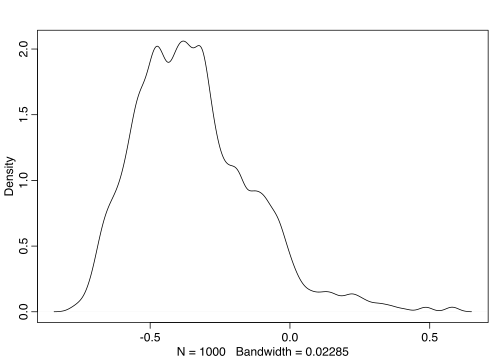
\includegraphics{17_brms_files/figure-latex/unnamed-chunk-224-1.pdf}

\begin{Shaded}
\begin{Highlighting}[]
\KeywordTok{plot}\NormalTok{(}\KeywordTok{marginal_effects}\NormalTok{(ln_m1, }\DataTypeTok{method=}\StringTok{"predict"}\NormalTok{), }\DataTypeTok{points=}\OtherTok{TRUE}\NormalTok{)}
\end{Highlighting}
\end{Shaded}

\includegraphics{17_brms_files/figure-latex/unnamed-chunk-225-1.pdf}

\begin{Shaded}
\begin{Highlighting}[]
\NormalTok{ln_m2 <-}\StringTok{ }\KeywordTok{brm}\NormalTok{(l_GDP}\OperatorTok{~}\NormalTok{lifeExp, }\DataTypeTok{data=}\NormalTok{g2007, }\DataTypeTok{cores=}\DecValTok{4}\NormalTok{)}
\KeywordTok{write_rds}\NormalTok{(ln_m2, }\StringTok{"ln_m2.rds"}\NormalTok{)}
\end{Highlighting}
\end{Shaded}

\begin{Shaded}
\begin{Highlighting}[]
\NormalTok{ln_m2 <-}\StringTok{ }\KeywordTok{read_rds}\NormalTok{(}\StringTok{"ln_m2.rds"}\NormalTok{)}
\end{Highlighting}
\end{Shaded}

\begin{Shaded}
\begin{Highlighting}[]
\KeywordTok{plot}\NormalTok{(}\KeywordTok{marginal_effects}\NormalTok{(ln_m2, }\DataTypeTok{method=}\StringTok{"predict"}\NormalTok{), }\DataTypeTok{points=}\OtherTok{TRUE}\NormalTok{)}
\end{Highlighting}
\end{Shaded}

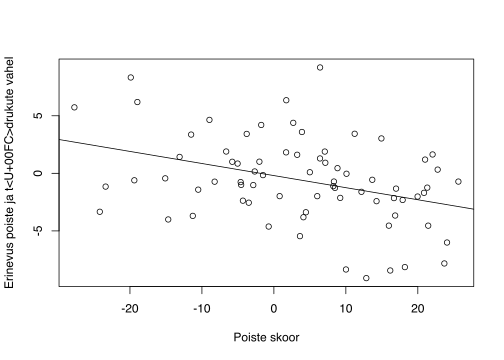
\includegraphics{17_brms_files/figure-latex/unnamed-chunk-228-1.pdf}

\begin{Shaded}
\begin{Highlighting}[]
\KeywordTok{bayes_R2}\NormalTok{(ln_m1)}
\end{Highlighting}
\end{Shaded}

\begin{verbatim}
##     Estimate  Est.Error      Q2.5     Q97.5
## R2 0.5869887 0.07670807 0.4288752 0.7269154
\end{verbatim}

\begin{Shaded}
\begin{Highlighting}[]
\KeywordTok{bayes_R2}\NormalTok{(ln_m2)}
\end{Highlighting}
\end{Shaded}

\begin{verbatim}
##     Estimate  Est.Error     Q2.5     Q97.5
## R2 0.6516089 0.02771113 0.589718 0.6975756
\end{verbatim}

\begin{Shaded}
\begin{Highlighting}[]
\KeywordTok{plot}\NormalTok{(}\KeywordTok{marginal_effects}\NormalTok{(ln_m2), }\DataTypeTok{points=}\OtherTok{TRUE}\NormalTok{)}
\end{Highlighting}
\end{Shaded}

\includegraphics{17_brms_files/figure-latex/unnamed-chunk-231-1.pdf}

\subsubsection{Puuduvate andmete
imputatsioon}\label{puuduvate-andmete-imputatsioon}

Regressioonimudelite fittimisel kasutatakse ainult vaatlusi, kus
esinevad väärtused kõigis mudelisse pandud muutujates. Seega, kui meil
on palju muutujaid, milles igaühes puuduvad juhuslikult mõned väärtused,
siis kaotame kokkuvõttes enamuse oma valimist. Aitab puuduvate andmete
imputatsioon, mis tegelikult tähendab, et me fitime iga puuduvaid
andmeid sisaldava muutuja eraldi regressioonimudelis kõigi teiste
muutujate vastu.

Eriti vajalik, kui andmed ei puudu juhuslikult!

Viskame irise andmestiku kahest tulbast välja 1/4 andmepunkte, aga mitte
juhuslikult vaid kõik madalamad väärtused. Selline suunatud tegevus
kallutab (ehk suunab kindlas suunas) oluliselt mudeldamise tulemusi

\begin{Shaded}
\begin{Highlighting}[]
\KeywordTok{quantile}\NormalTok{(iris}\OperatorTok{$}\NormalTok{Petal.Length)}
\end{Highlighting}
\end{Shaded}

\begin{verbatim}
##   0%  25%  50%  75% 100% 
## 1.00 1.60 4.35 5.10 6.90
\end{verbatim}

\begin{Shaded}
\begin{Highlighting}[]
\NormalTok{iris_na <-}\StringTok{ }\NormalTok{iris}
\NormalTok{iris_na}\OperatorTok{$}\NormalTok{Sepal.Length[iris_na}\OperatorTok{$}\NormalTok{Sepal.Length }\OperatorTok{<}\StringTok{ }\DecValTok{5}\NormalTok{] <-}\StringTok{ }\OtherTok{NA}
\NormalTok{iris_na}\OperatorTok{$}\NormalTok{Petal.Length[iris_na}\OperatorTok{$}\NormalTok{Petal.Length }\OperatorTok{<}\StringTok{ }\FloatTok{1.6}\NormalTok{] <-}\StringTok{ }\OtherTok{NA}
\end{Highlighting}
\end{Shaded}

\begin{Shaded}
\begin{Highlighting}[]
\KeywordTok{lm}\NormalTok{(Petal.Length }\OperatorTok{~}\StringTok{ }\NormalTok{Sepal.Length, }\DataTypeTok{data =}\NormalTok{ iris) }\OperatorTok\StringTok{ }\KeywordTok{tidy}\NormalTok{()}
\end{Highlighting}
\end{Shaded}

\begin{verbatim}
## # A tibble: 2 x 5
##   term         estimate std.error statistic  p.value
##   <chr>           <dbl>     <dbl>     <dbl>    <dbl>
## 1 (Intercept)     -7.10    0.507      -14.0 6.13e-29
## 2 Sepal.Length     1.86    0.0859      21.6 1.04e-47
\end{verbatim}

\begin{Shaded}
\begin{Highlighting}[]
\KeywordTok{lm}\NormalTok{(Petal.Length }\OperatorTok{~}\StringTok{ }\NormalTok{Sepal.Length, }\DataTypeTok{data =}\NormalTok{ iris_na) }\OperatorTok\StringTok{ }\KeywordTok{tidy}\NormalTok{()}
\end{Highlighting}
\end{Shaded}

\begin{verbatim}
## # A tibble: 2 x 5
##   term         estimate std.error statistic  p.value
##   <chr>           <dbl>     <dbl>     <dbl>    <dbl>
## 1 (Intercept)     -4.19    0.609      -6.89 4.33e-10
## 2 Sepal.Length     1.43    0.0976     14.6  4.53e-27
\end{verbatim}

imputeerime enne mudeli fittimist kasutades multiple imputation meetodit
mice paketist \url{https://stefvanbuuren.name/mice/}. Siin imputeerime
iga puuduva väärtuse kasutades kõigi teiste parameetrite väärtusi, ja me
teeme seda 5 korda.

\begin{Shaded}
\begin{Highlighting}[]
\KeywordTok{library}\NormalTok{(mice)}
\NormalTok{imp <-}\StringTok{ }\KeywordTok{mice}\NormalTok{(iris_na, }\DataTypeTok{m =} \DecValTok{5}\NormalTok{, }\DataTypeTok{print =} \OtherTok{FALSE}\NormalTok{)}
\end{Highlighting}
\end{Shaded}

Meil on nüüd 5 imputeeritud andmesetti. Me saadame need kõik brms-i.

\begin{quote}
Siin kasutame mice() tema vaikeväärtustel, kuid mice pakett on
tegelikult vägagi rikkalik imputatsioonimasin, mille helpi ja
tutoorialeid tuleks kindlasti enne lugeda, kui oma andmeid imputeerima
asuda. Lisaks, see raamat on tervenisti pühendatud imputatsioonile:
\url{https://stefvanbuuren.name/fimd/}
\end{quote}

\begin{Shaded}
\begin{Highlighting}[]
\NormalTok{iris_imp1 <-}\StringTok{ }\KeywordTok{brm_multiple}\NormalTok{(Petal.Length }\OperatorTok{~}\StringTok{ }\NormalTok{Sepal.Length, }\DataTypeTok{data =}\NormalTok{ imp)}
\KeywordTok{write_rds}\NormalTok{(iris_imp1, }\DataTypeTok{path =} \StringTok{"data/iris_imp1.fit"}\NormalTok{)}
\end{Highlighting}
\end{Shaded}

Saame tavalise fitiobjekti, kus on 5 alammudeli posterioorid. Kõik juba
koos.

\begin{Shaded}
\begin{Highlighting}[]
\KeywordTok{tidy}\NormalTok{(iris_imp1)[,}\DecValTok{1}\OperatorTok{:}\DecValTok{3}\NormalTok{]}
\end{Highlighting}
\end{Shaded}

\begin{verbatim}
##             term     estimate  std.error
## 1    b_Intercept   -7.6920342 0.55428281
## 2 b_Sepal.Length    1.9482798 0.09293763
## 3          sigma    0.8432503 0.05234786
## 4           lp__ -192.5742084 3.25012585
\end{verbatim}

Tõepoolest, süstemaatiliselt rikutud andmetest on imutatsiooni abil
võimalik täitsa head ennustust tagasi saada!!!

\subsection{Imputatsioon otse brms-is}\label{imputatsioon-otse-brms-is}

See töötab küll irise peal halvemini kui mice!

\begin{Shaded}
\begin{Highlighting}[]
\NormalTok{bform <-}\StringTok{ }\KeywordTok{bf}\NormalTok{(Petal.Length }\OperatorTok{|}\StringTok{ }\KeywordTok{mi}\NormalTok{() }\OperatorTok{~}\StringTok{ }\KeywordTok{mi}\NormalTok{(Sepal.Length)) }\OperatorTok{+}\StringTok{ }
\StringTok{  }\KeywordTok{bf}\NormalTok{(Sepal.Length }\OperatorTok{|}\StringTok{ }\KeywordTok{mi}\NormalTok{() }\OperatorTok{~}\StringTok{ }\NormalTok{Sepal.Width }\OperatorTok{+}\StringTok{ }\NormalTok{Petal.Width }\OperatorTok{+}\StringTok{ }\NormalTok{Species }\OperatorTok{+}\StringTok{ }\KeywordTok{mi}\NormalTok{(Petal.Length)) }\OperatorTok{+}\StringTok{ }\KeywordTok{set_rescor}\NormalTok{(}\OtherTok{FALSE}\NormalTok{)}
\NormalTok{iris_imp2 <-}\StringTok{ }\KeywordTok{brm}\NormalTok{(bform, }\DataTypeTok{data =}\NormalTok{ iris_na)}
\KeywordTok{write_rds}\NormalTok{(iris_imp2, }\DataTypeTok{path =} \StringTok{"data/iris_imp2.fit"}\NormalTok{)}
\end{Highlighting}
\end{Shaded}

Kasutades mi() funktsiooni peame siin ekslpitsiitselt ütlema, milliseid
muutujaid soovime imputeerida. Me imputeerime Petal.Length-i, kasutades
NA-de väärtuste prediktorina Sepal.Length-i, mis on omakorda
imputeeritud. Sepal.Length-i imputeerime omakorda Sepal.Width,
Petal.width jne järgi.

\begin{Shaded}
\begin{Highlighting}[]
\NormalTok{bform <-}\StringTok{ }\KeywordTok{bf}\NormalTok{(Petal.Length }\OperatorTok{|}\StringTok{ }\KeywordTok{mi}\NormalTok{() }\OperatorTok{~}\StringTok{ }\KeywordTok{mi}\NormalTok{(Sepal.Length)) }\OperatorTok{+}\StringTok{ }
\StringTok{  }\KeywordTok{bf}\NormalTok{(Sepal.Length }\OperatorTok{|}\StringTok{ }\KeywordTok{mi}\NormalTok{() }\OperatorTok{~}\StringTok{ }\NormalTok{Species) }\OperatorTok{+}\StringTok{ }\KeywordTok{set_rescor}\NormalTok{(}\OtherTok{FALSE}\NormalTok{)}
\NormalTok{iris_imp3 <-}\StringTok{ }\KeywordTok{brm}\NormalTok{(bform, }\DataTypeTok{data =}\NormalTok{ iris_na)}
\KeywordTok{write_rds}\NormalTok{(iris_imp3, }\DataTypeTok{path =} \StringTok{"data/iris_imp3.fit"}\NormalTok{)}
\end{Highlighting}
\end{Shaded}

\begin{Shaded}
\begin{Highlighting}[]
\KeywordTok{tidy}\NormalTok{(iris_imp2) }\OperatorTok\StringTok{ }\KeywordTok{head}\NormalTok{()}
\end{Highlighting}
\end{Shaded}

\begin{verbatim}
##                              term   estimate  std.error      lower
## 1         b_PetalLength_Intercept -5.5689751 0.49166142 -6.2043923
## 2         b_SepalLength_Intercept  2.6008323 0.32550167  2.1146496
## 3       b_SepalLength_Sepal.Width  0.3073513 0.08550384  0.1636517
## 4       b_SepalLength_Petal.Width  0.0679416 0.15154905 -0.1302599
## 5 b_SepalLength_Speciesversicolor -0.2201413 0.15949098 -0.4822360
## 6  b_SepalLength_Speciesvirginica -0.4502161 0.23186720 -0.8562267
##         upper
## 1 -4.81286282
## 2  3.12461170
## 3  0.42965995
## 4  0.33296059
## 5  0.01717628
## 6 -0.09367050
\end{verbatim}

\begin{Shaded}
\begin{Highlighting}[]
\KeywordTok{tidy}\NormalTok{(iris_imp3) }\OperatorTok\StringTok{ }\KeywordTok{head}\NormalTok{()}
\end{Highlighting}
\end{Shaded}

\begin{verbatim}
##                              term   estimate  std.error      lower
## 1         b_PetalLength_Intercept -4.6011422 0.58642627 -5.5603660
## 2         b_SepalLength_Intercept  5.1680100 0.09148933  5.0143264
## 3 b_SepalLength_Speciesversicolor  0.7809822 0.11573409  0.5903730
## 4  b_SepalLength_Speciesvirginica  1.4494074 0.11550544  1.2587559
## 5  bsp_PetalLength_miSepal.Length  1.4881584 0.09447771  1.3334928
## 6               sigma_PetalLength  0.7053926 0.04935572  0.6297299
##        upper
## 1 -3.6498716
## 2  5.3161878
## 3  0.9707784
## 4  1.6448384
## 5  1.6424317
## 6  0.7905259
\end{verbatim}

\subsection{Binoomjaotusega mudelid}\label{binoomjaotusega-mudelid}

y ∼ Binomial(n,p)

Me teeme n katset ja kodeerime iga eduka katse 1-ga ja mitteeduka katse
0-ga. Kui n=1, siis y on ühtedest ja nullidest koosnev vektor (muutuja)
ja p on tõenäosus, et suvaline katse annab tulemuseks 1-e. Eeldades
logistilist transformatsiooni on siin tegu logistilise regressiooniga.
Kui n \textgreater{} 1 (ja ikka eeldades logistilist transformatsiooni),
siis on tegu aggregeeritud binoomse logistilise regressiooniga. Me
lahendame allpool need mõlemad.

\subsubsection{Logistiline regressioon}\label{logistiline-regressioon}

Tavalises lineaarses regressioonis on tavapärane, et kuigi me ennustame
pidevat y-muutujat, kas osad või kõik X-muutujad (prediktorid) on
mittepidevad. Lineaarsed mudelid jooksevad võrdselt hästi pidevate ja
mittepidevate (binaarsete) prediktoritega. (Binaarsed muutujad võivad
omada kaht diskreetset väärtust, mida kodeerime 1 ja 0-na). Aga kuidas
käituda, kui meie poolt ennustatav Y-muutuja on binaarne? Kui me püüame
ennustada binaarse y-muutuja oodatavaid väärtusi tõenäosustena, ehk 1-de
arvu suhet katsete koguarvu, kas siis tavaline lineaarne regressioon
enam ei tööta? Töötab küll, aga paraku ei ole garanteeritud, et mudeli
ennustused jäävad 0 ja 1 vahele, ehk tõenäosuste skaalasse. Seda tagab
logistiline regressioon. Logistilises regressioonis ei modelleeri me
mitte otse y väärtusi (1 ja 0) erinevatel x-i väärtustel, vaid
tõenäosust P(Y = 1 \textbar{} X) {[}tõenäosus, et Y = 1, fikseeritud x-i
väärtusel{]}.

Logistiline regressioon töötab tänu logistilisele transformatsioonile.
Näiteks logistiline transformatsioon funktsioonile \(y = a + bx\) näeb
välja niimoodi \[y=\frac{exp(a + bx)}{1 + exp(a + bx)}\]

\begin{verbatim}
exp(a) tähendab "e astmes a", kus e on Euleri arv, ehk arv, mille 
naturaal-logaritm = 1 (seega on e naturaal-logaritmi alus). 
e on umbes 2.71828 ja selle saab valemist (1 + 1/n)^n, 
kui n läheneb lõpmatusele.
\end{verbatim}

\paragraph{Logistiline ja logit transformatsioon -
definitsioonid}\label{logistiline-ja-logit-transformatsioon---definitsioonid}

See peatükk aitab loogilisest regressioonist aru saada - aru saamine
pole aga tingimata vajalik selle edukaks tegemiseks.

Logistiline transformatsioon viib lineaarse regressiooni tavapärasest
y-muutuja skaalast {[}−∞,+∞{]} tõenäosuste skaalasse {[}0,1{]}, andes
meile sirge asemele S-kujulise kurvi, mis läheneb asümptootiliselt ühelt
poolt 0-le ja teiselt poolt 1-le. Logistilise funktsiooni põõrdväärtus
on logit funktsioon, mis annab ``\emph{odds}-i'' ehk shansi ehk
kihlveosuhted tõenäosusele p: \(odds = \frac {p}{1 − p}\). Tõenäosuse p
logit ehk logit(p) on sama, mis log(odds):

\[logit(p)=\log \left({\frac {p}{1-p}}\right)=\log(p)-\log(1-p)\]

Meie y = a + bx mudeli korral tavalises meetrilises skaalas on
\emph{odds} exponent meie fititud lineaarsest mudelist:

\[odds= \frac {P(Y = 1 ~|~ X)}{1-P(Y = 1 ~|~ X)} = exp(a+bx)\]

Näiteks tõenäosus 0.2 (20\%) tähendab, et \(odds = 0.2/(1 - 0.2) = 1/4\)
ehk üks neljale ja tõenäosus 0.9 tähendab, et
\(odds = 0.9/(1 - 0.9) = 9\) ehk üheksa ühele. Sellel meetodil töötavad
näiteks hipodroomid, sest nii on mänguril lihtne näha, et kui
kihlveokontori poolt mingile hobusele omistatud odds on näiteks üks
nelja vastu ja te maksate kihlveo maaklerile 1 euro, siis saab võidu
korral 4 eurot kasumit (ehk 5 eurose kupüüri). Logaritm
\emph{odds}-idest ongi logit transformatsioon, mille pöördväärtus on
omakorda logistiline transformatsioon!

Suvalise arvu α logistiline funktsioon on logiti põõrdväärtus:

\[logit^{-1}\alpha=logistic (\alpha)={\frac {exp (\alpha) }{1+ exp (\alpha)}}\]

\begin{Shaded}
\begin{Highlighting}[]
\NormalTok{x <-}\StringTok{ }\OperatorTok{-}\DecValTok{10}\OperatorTok{:}\DecValTok{10}
\NormalTok{y <-}\StringTok{ }\KeywordTok{exp}\NormalTok{(x)}\OperatorTok{/}\NormalTok{(}\DecValTok{1}\OperatorTok{+}\KeywordTok{exp}\NormalTok{(x))}
\KeywordTok{plot}\NormalTok{(y}\OperatorTok{~}\NormalTok{x)}
\end{Highlighting}
\end{Shaded}

\includegraphics{17_brms_files/figure-latex/unnamed-chunk-244-1.pdf}

Kui me mudeli y = a + bx korral muudame x-i ühe ühiku võrra muutuvad
log-odds-id b võrra. Teisisõnu võime korrutada lineaarses skaalas
\emph{odds}-id exp(b)-ga. Kuna P(Y = 1 \textbar{} X) ja X-i seos ei ole
sirge, siis b ei vasta P(Y = 1 \textbar{} X) muutusele X-i muutumisel
ühe ühiku võrra. See, kui kiiresti P(Y = 1 \textbar{} X) muutub, sõltub
X-i väärtusest, aga hoolimata sellest, senikaua kui b \textgreater{} 0,
on X-i kasv alati seotud tõenäosuse kasvuga (ja vastupidi).

Kahe tõenäosuse logitite vahe on sama, mis logaritm \emph{odds-ratio}-st
(log(OR) ehk shanside suhe)

\[{log} (OR)= {logit} (p_{1})- {logit} (p_{2})\]

\textbf{Odds-ratio}

Kui meil on 2 katsetingimust (ravim/platseebo) ning 2 väljundit (näit
elus/surnud), siis

\begin{itemize}
\item
  a - ravim/elus juhutude arv,
\item
  b - ravim/surnud juhutude arv,
\item
  c - platseebo/elus juhutude arv,
\item
  d - platseebo/surnud juhutude arv.
\end{itemize}

\[OR = \frac {a/b}{c/d}\]

\begin{itemize}
\item
  OR = 1 Katsetingimus ei mõjuta väljundi \emph{odds}-e
\item
  OR \textgreater{} 1 Katsetingimus tõstab väljundi \emph{odds}-e
\item
  OR \textless{} 1 Katsetingimus langetab väljundi \emph{odds}-e
\end{itemize}

Logistiline regressioon üldistab OR-i kaugemale 2st binaarsest
muutujast. Kui meil on binaarne y-muutuja ja binaarne x-muutuja (x1),
pluss rida teisi x-muutujaid (x2\ldots{}xn), siis mitmese logistilise
regressiooni x1-e tõusukoefitsient b1 on seotud tingimusliku OR-ga.
\(\exp(\beta_1)\) annab Y ja X vahelise OR-i, tingimusel, et teiste
x-muutujate väärtused on fikseeritud (see on tavaline sõltumatute
muutujatega lineaarse regressiooni beta-koefitsientide tõlgendamise
tingimus).

\begin{verbatim}
OR-i kui suhtelise efekti suuruse tõlgendamine sõltub sündmuse y = 1 
baastõenäosusest. Näiteks kui surm põhjusel x on tavapäraselt väga 
haruldane ja mingi keskkonnamõju annab OR = 10, siis tegelik tõus 
suremuses (surma tõenäosus keskkonnamõju tingimustes) võib olla tühine. 
\end{verbatim}

\paragraph{Logistiline regressioon
brms-s}\label{logistiline-regressioon-brms-s}

\begin{Shaded}
\begin{Highlighting}[]
\KeywordTok{library}\NormalTok{(rethinking)}
\end{Highlighting}
\end{Shaded}

\begin{Shaded}
\begin{Highlighting}[]
\KeywordTok{data}\NormalTok{(chimpanzees)}
\KeywordTok{skim}\NormalTok{(chimpanzees)}
\end{Highlighting}
\end{Shaded}

\begin{verbatim}
## Skim summary statistics
##  n obs: 504 
##  n variables: 8 
## 
## -- Variable type:integer ----------------------------------------------
##      variable missing complete   n  mean    sd p0 p25  p50 p75 p100
##         actor       0      504 504  4     2     1   2  4     6    7
##         block       0      504 504  3.5   1.71  1   2  3.5   5    6
##  chose_prosoc       0      504 504  0.57  0.5   0   0  1     1    1
##     condition       0      504 504  0.5   0.5   0   0  0.5   1    1
##   prosoc_left       0      504 504  0.5   0.5   0   0  0.5   1    1
##   pulled_left       0      504 504  0.58  0.49  0   0  1     1    1
##     recipient     252      252 504  5     2     2   3  5     7    8
##         trial       0      504 504 36.38 20.79  1  18 36    54   72
##      hist
##  ▇▇▇▇▁▇▇▇
##  ▇▇▁▇▇▁▇▇
##  ▆▁▁▁▁▁▁▇
##  ▇▁▁▁▁▁▁▇
##  ▇▁▁▁▁▁▁▇
##  ▆▁▁▁▁▁▁▇
##  ▇▇▇▇▁▇▇▇
##  ▇▇▇▇▇▇▇▇
\end{verbatim}

\paragraph{Intercept only model}\label{intercept-only-model}

\begin{Shaded}
\begin{Highlighting}[]
\NormalTok{m_logreg_}\DecValTok{1}\NormalTok{ <-}\StringTok{ }\KeywordTok{brm}\NormalTok{(}\DataTypeTok{data =}\NormalTok{ chimpanzees, }
                  \DataTypeTok{family =}\NormalTok{ binomial,}
\NormalTok{                  pulled_left }\OperatorTok{~}\StringTok{ }\DecValTok{1}\NormalTok{,}
                  \KeywordTok{prior}\NormalTok{(}\KeywordTok{normal}\NormalTok{(}\DecValTok{0}\NormalTok{, }\DecValTok{10}\NormalTok{), }\DataTypeTok{class =}\NormalTok{ Intercept))}
\KeywordTok{write_rds}\NormalTok{(m_logreg_}\DecValTok{1}\NormalTok{, }\DataTypeTok{path=} \StringTok{"data/m_logreg_1.fit"}\NormalTok{)}
\end{Highlighting}
\end{Shaded}

\begin{Shaded}
\begin{Highlighting}[]
\NormalTok{m_logreg_}\DecValTok{1}\NormalTok{ <-}\StringTok{ }\KeywordTok{read_rds}\NormalTok{(}\StringTok{"data/m_logreg_1.fit"}\NormalTok{)}
\end{Highlighting}
\end{Shaded}

\begin{Shaded}
\begin{Highlighting}[]
\KeywordTok{tidy}\NormalTok{(m_logreg_}\DecValTok{1}\NormalTok{)}
\end{Highlighting}
\end{Shaded}

\begin{verbatim}
##          term     estimate  std.error       lower        upper
## 1 b_Intercept    0.3229989 0.08815701    0.180684    0.4641893
## 2        lp__ -346.6692033 0.66518291 -347.959467 -346.1939464
\end{verbatim}

Tõenäosus, et shimpans ``pulled left'':

\begin{Shaded}
\begin{Highlighting}[]
\KeywordTok{inv_logit_scaled}\NormalTok{(}\KeywordTok{fixef}\NormalTok{(m_logreg_}\DecValTok{1}\NormalTok{))}
\end{Highlighting}
\end{Shaded}

\begin{verbatim}
##            Estimate Est.Error      Q2.5     Q97.5
## Intercept 0.5800549  0.522025 0.5386246 0.6211881
\end{verbatim}

See tõenäosus peaks seega jääma kuhugi 54\% ja 62\% vahele.

Nüüd ehtne ennustav logistiline regressioonimudel

\begin{Shaded}
\begin{Highlighting}[]
\NormalTok{m_logreg_}\DecValTok{2}\NormalTok{ <-}
\StringTok{  }\KeywordTok{brm}\NormalTok{(}\DataTypeTok{data =}\NormalTok{ d, }\DataTypeTok{family =}\NormalTok{ binomial,}
\NormalTok{      pulled_left }\OperatorTok{~}\StringTok{ }\DecValTok{1} \OperatorTok{+}\StringTok{ }\NormalTok{prosoc_left,}
      \DataTypeTok{prior =} \KeywordTok{c}\NormalTok{(}\KeywordTok{prior}\NormalTok{(}\KeywordTok{normal}\NormalTok{(}\DecValTok{0}\NormalTok{, }\DecValTok{10}\NormalTok{), }\DataTypeTok{class =}\NormalTok{ Intercept),}
                \KeywordTok{prior}\NormalTok{(}\KeywordTok{normal}\NormalTok{(}\DecValTok{0}\NormalTok{, }\DecValTok{10}\NormalTok{), }\DataTypeTok{class =}\NormalTok{ b)))}
\KeywordTok{write_rds}\NormalTok{(m_logreg_}\DecValTok{2}\NormalTok{, }\DataTypeTok{path=} \StringTok{"data/m_logreg_2.fit"}\NormalTok{)}
\end{Highlighting}
\end{Shaded}

\begin{Shaded}
\begin{Highlighting}[]
\NormalTok{m_logreg_}\DecValTok{2}\NormalTok{ <-}\StringTok{ }\KeywordTok{read_rds}\NormalTok{(}\StringTok{"data/m_logreg_2.fit"}\NormalTok{)}
\end{Highlighting}
\end{Shaded}

\begin{Shaded}
\begin{Highlighting}[]
\KeywordTok{tidy}\NormalTok{(m_logreg_}\DecValTok{2}\NormalTok{)}
\end{Highlighting}
\end{Shaded}

\begin{verbatim}
##            term      estimate std.error        lower        upper
## 1   b_Intercept    0.04562136 0.1277891   -0.1654294    0.2586237
## 2 b_prosoc_left    0.56590225 0.1870018    0.2597061    0.8785781
## 3          lp__ -345.71023786 1.0144730 -347.6393646 -344.7413692
\end{verbatim}

The proportional odds = 1.76, which is the ratio of the probability an
event happens to the probability it does not happen (the outcome or y
variable).

If changing the predictor prosoc\_left from 0 to 1 increases the
log-odds of pulling the left-hand lever by 0.57, then there is a
proportional increase of exp(0.57) = 1.76 in the odds of pulling the
left-hand lever. This means that the odds increase by 73\%.

\begin{Shaded}
\begin{Highlighting}[]
\KeywordTok{exp}\NormalTok{(}\FloatTok{0.57}\NormalTok{)}
\end{Highlighting}
\end{Shaded}

\begin{verbatim}
## [1] 1.768267
\end{verbatim}

The actual change in probability will also depend upon the intercept,
alpha, as well as any other predictor variables. Logistic regression
induce interactions among all variables. You can think of these
interactions as resulting from both ceiling and floor effects: If the
intercept is large enough to guarantee a pull, then increasing the odds
by 73\% isn't going to make it any more guaranteed. Suppose α = 4. Then
the probability of a pull, ignoring everything else, would be
\texttt{inv\_logit\_scaled(4)} = 0.98. Adding in an increase of 0.57
(the estimate for beta) changes this to:
\texttt{inv\_logit\_scaled(4\ +\ 0.57)} = 0.99. That's a difference, on
the absolute scale, of 1\%, despite being an 73\% increase in
proportional odds. Likewise, if the intercept is very negative, then the
probability of a pull is almost zero. An increase in odds of 73\% may
not be enough to get the probability up from the floor.

\begin{Shaded}
\begin{Highlighting}[]
\KeywordTok{inv_logit_scaled}\NormalTok{(}\FloatTok{0.04562136} \OperatorTok{+}\StringTok{ }\FloatTok{0.56590225}\NormalTok{)}
\end{Highlighting}
\end{Shaded}

\begin{verbatim}
## [1] 0.6482883
\end{verbatim}

Pr of pulling left, if prosoc\_left is 1, is 64\%.

\begin{Shaded}
\begin{Highlighting}[]
\KeywordTok{inv_logit_scaled}\NormalTok{(}\FloatTok{0.04562136}\NormalTok{)}
\end{Highlighting}
\end{Shaded}

\begin{verbatim}
## [1] 0.5114034
\end{verbatim}

If prosoc\_left is 0, it is 51\%.

This meagre difference is reflected in the roc curve.

\begin{Shaded}
\begin{Highlighting}[]
\NormalTok{glm.probs <-}\StringTok{ }\KeywordTok{predict}\NormalTok{(m_logreg_}\DecValTok{2}\NormalTok{, }\DataTypeTok{type =} \StringTok{"response"}\NormalTok{) }\OperatorTok\StringTok{ }\KeywordTok{as.data.frame}\NormalTok{()}
\end{Highlighting}
\end{Shaded}

\begin{verbatim}
## Using the maximum response value as the number of trials.
\end{verbatim}

\begin{Shaded}
\begin{Highlighting}[]
\NormalTok{glm.probs <-}\StringTok{ }\NormalTok{glm.probs[,}\DecValTok{1}\NormalTok{]}
\NormalTok{glm.pred <-}\StringTok{ }\KeywordTok{rep}\NormalTok{(}\StringTok{"pulled_right"}\NormalTok{, }\DecValTok{504}\NormalTok{)}
\NormalTok{glm.pred[glm.probs }\OperatorTok{>}\StringTok{ }\FloatTok{0.5}\NormalTok{] <-}\StringTok{ "pulled_left"} 
\KeywordTok{table}\NormalTok{(glm.pred, chimpanzees}\OperatorTok{$}\NormalTok{pulled_left)}
\end{Highlighting}
\end{Shaded}

\begin{verbatim}
##               
## glm.pred         0   1
##   pulled_left  202 279
##   pulled_right  10  13
\end{verbatim}

\begin{Shaded}
\begin{Highlighting}[]
\KeywordTok{library}\NormalTok{(pROC)}
\NormalTok{roccurve <-}\StringTok{ }\KeywordTok{roc}\NormalTok{(chimpanzees}\OperatorTok{$}\NormalTok{pulled_left }\OperatorTok{~}\StringTok{ }\NormalTok{glm.probs)}
\KeywordTok{plot}\NormalTok{(roccurve, }\DataTypeTok{legacy.axes =} \OtherTok{TRUE}\NormalTok{, }\DataTypeTok{cex.axis =} \FloatTok{0.7}\NormalTok{, }\DataTypeTok{cex.lab =} \FloatTok{0.8}\NormalTok{)}
\end{Highlighting}
\end{Shaded}

\includegraphics{17_brms_files/figure-latex/unnamed-chunk-258-1.pdf}

Sarnase mudeli saab fittida ka siis, kui n\textgreater{}1 ja meil on
igale ahvile countide suhted nr of pull-left/total pulls. Nüüd on meil
vaja lisada trials(), kuhu läheb n kas ühe numbrina või muutujana, mis
indekseerib sündmuste arvu ehk n-i. Antud juhul on kõikidel ahvidel
katsete arv n 18.

\begin{Shaded}
\begin{Highlighting}[]
\NormalTok{chimp_aggr <-}\StringTok{ }\KeywordTok{select}\NormalTok{(chimpanzees, actor, condition, prosoc_left, pulled_left) }\OperatorTok
\StringTok{  }\KeywordTok{group_by}\NormalTok{(actor, condition, prosoc_left) }\OperatorTok
\StringTok{  }\KeywordTok{summarise_at}\NormalTok{(}\StringTok{"pulled_left"}\NormalTok{, sum)}
\NormalTok{m_logreg_}\DecValTok{3}\NormalTok{ <-}\StringTok{ }\KeywordTok{brm}\NormalTok{(pulled_left }\OperatorTok{|}\StringTok{ }\KeywordTok{trials}\NormalTok{(}\DecValTok{18}\NormalTok{) }\OperatorTok{~}\StringTok{ }\DecValTok{1} \OperatorTok{+}\StringTok{ }\NormalTok{prosoc_left, }
                  \DataTypeTok{data =}\NormalTok{ chimp_aggr, }
                  \DataTypeTok{family =}\NormalTok{ binomial)}
\end{Highlighting}
\end{Shaded}

Koefitsendid tulevad samad, mis eelmisel mudelil.

Näide agregeeritud binoomsetele andmetele.

\begin{Shaded}
\begin{Highlighting}[]
\KeywordTok{data}\NormalTok{(UCBadmit)}
\KeywordTok{head}\NormalTok{(UCBadmit)}
\end{Highlighting}
\end{Shaded}

\begin{verbatim}
##   dept applicant.gender admit reject applications
## 1    A             male   512    313          825
## 2    A           female    89     19          108
## 3    B             male   353    207          560
## 4    B           female    17      8           25
## 5    C             male   120    205          325
## 6    C           female   202    391          593
\end{verbatim}

\begin{Shaded}
\begin{Highlighting}[]
\NormalTok{ucbadmit <-}\StringTok{ }\KeywordTok{mutate}\NormalTok{(UCBadmit, }\DataTypeTok{male =} \KeywordTok{case_when}\NormalTok{(}
\NormalTok{  applicant.gender }\OperatorTok{==}\StringTok{ "male"} \OperatorTok{~}\StringTok{ }\DecValTok{1}\NormalTok{,}
  \OtherTok{TRUE} \OperatorTok{~}\StringTok{ }\DecValTok{0}
\NormalTok{))}
\end{Highlighting}
\end{Shaded}

\begin{Shaded}
\begin{Highlighting}[]
\NormalTok{m_ucadmit1 <-}\StringTok{ }\KeywordTok{brm}\NormalTok{(admit }\OperatorTok{|}\StringTok{ }\KeywordTok{trials}\NormalTok{(applications) }\OperatorTok{~}\StringTok{ }\DecValTok{1} \OperatorTok{+}\StringTok{ }\NormalTok{male,}
                  \DataTypeTok{data =}\NormalTok{ ubcadmit, }
                  \DataTypeTok{family =}\NormalTok{ binomial,}
                  \DataTypeTok{prior =} \KeywordTok{c}\NormalTok{(}\KeywordTok{prior}\NormalTok{(}\KeywordTok{normal}\NormalTok{(}\DecValTok{0}\NormalTok{, }\DecValTok{10}\NormalTok{), }\DataTypeTok{class =}\NormalTok{ Intercept), }
                            \KeywordTok{prior}\NormalTok{(}\KeywordTok{normal}\NormalTok{(}\DecValTok{0}\NormalTok{, }\DecValTok{10}\NormalTok{), }\DataTypeTok{class =}\NormalTok{ b)))}
\KeywordTok{write_rds}\NormalTok{(m_ucadmit1, }\DataTypeTok{path =} \StringTok{"data/m_ucadmit1.fit"}\NormalTok{)}
\end{Highlighting}
\end{Shaded}

\begin{Shaded}
\begin{Highlighting}[]
\NormalTok{m_ucadmit1 <-}\StringTok{ }\KeywordTok{read_rds}\NormalTok{(}\StringTok{"data/m_ucadmit1.fit"}\NormalTok{)}
\end{Highlighting}
\end{Shaded}

\begin{Shaded}
\begin{Highlighting}[]
\KeywordTok{tidy}\NormalTok{(m_ucadmit1)}
\end{Highlighting}
\end{Shaded}

\begin{verbatim}
##          term     estimate  std.error        lower        upper
## 1 b_Intercept   -0.8311433 0.05087528   -0.9175040   -0.7478350
## 2      b_male    0.6118988 0.06259961    0.5115236    0.7175192
## 3        lp__ -433.6945826 0.94842267 -435.6207322 -432.7763850
\end{verbatim}

\begin{Shaded}
\begin{Highlighting}[]
\KeywordTok{exp}\NormalTok{(}\FloatTok{0.61}\NormalTok{)}
\end{Highlighting}
\end{Shaded}

\begin{verbatim}
## [1] 1.840431
\end{verbatim}

Mehed saavad suhtelise 84\% eelise ülikooli sissesaamisel.

\begin{Shaded}
\begin{Highlighting}[]
\KeywordTok{inv_logit_scaled}\NormalTok{(}\OperatorTok{-}\FloatTok{0.83} \OperatorTok{+}\StringTok{ }\FloatTok{0.61}\NormalTok{)}
\end{Highlighting}
\end{Shaded}

\begin{verbatim}
## [1] 0.4452208
\end{verbatim}

Meeskandidaadi tõenäosus sisse saada on 44\%.

\begin{Shaded}
\begin{Highlighting}[]
\KeywordTok{inv_logit_scaled}\NormalTok{(}\OperatorTok{-}\FloatTok{0.83}\NormalTok{)}
\end{Highlighting}
\end{Shaded}

\begin{verbatim}
## [1] 0.3036451
\end{verbatim}

Naiskandidaadi tõenäosus sisse saada on 30\%.

Kui palju erinevad vastuvõtmise tõenäosused (usaldusintervallidega)?

\begin{Shaded}
\begin{Highlighting}[]
\NormalTok{post <-}\StringTok{ }\KeywordTok{posterior_samples}\NormalTok{(m_ucadmit1)}
\NormalTok{post }\OperatorTok\StringTok{ }\KeywordTok{mutate}\NormalTok{(}\DataTypeTok{p_admit_male =} \KeywordTok{inv_logit_scaled}\NormalTok{(b_Intercept }\OperatorTok{+}\StringTok{ }\NormalTok{b_male),}
                \DataTypeTok{p_admit_female =} \KeywordTok{inv_logit_scaled}\NormalTok{(b_Intercept),}
                \DataTypeTok{diff_admit =}\NormalTok{ p_admit_male }\OperatorTok{-}\StringTok{ }\NormalTok{p_admit_female) }\OperatorTok
\StringTok{  }\KeywordTok{summarise}\NormalTok{(}\StringTok{`}\DataTypeTok{2.5%}\StringTok{`}\NormalTok{  =}\StringTok{ }\KeywordTok{quantile}\NormalTok{(diff_admit, }\DataTypeTok{probs =}\NormalTok{ .}\DecValTok{025}\NormalTok{),}
            \StringTok{`}\DataTypeTok{50%}\StringTok{`}\NormalTok{   =}\StringTok{ }\KeywordTok{median}\NormalTok{(diff_admit),}
            \StringTok{`}\DataTypeTok{97.5%}\StringTok{`}\NormalTok{ =}\StringTok{ }\KeywordTok{quantile}\NormalTok{(diff_admit, }\DataTypeTok{probs =}\NormalTok{ .}\DecValTok{975}\NormalTok{))}
\end{Highlighting}
\end{Shaded}

\begin{verbatim}
##        2.5%       50%     97.5%
## 1 0.1151054 0.1419908 0.1701467
\end{verbatim}

Mudeldame otse küsimust, mis on naiste ja meeste erinevus sissesaamisel.
intercepti surume nulli, et saada eraldi hinnang igale departmendile:

\begin{Shaded}
\begin{Highlighting}[]
\NormalTok{m_ucadmit2 <-}\StringTok{ }\KeywordTok{brm}\NormalTok{(admit }\OperatorTok{|}\StringTok{ }\KeywordTok{trials}\NormalTok{(applications) }\OperatorTok{~}\StringTok{ }\DecValTok{0} \OperatorTok{+}\StringTok{ }\NormalTok{dept }\OperatorTok{+}\StringTok{ }\NormalTok{male,}
                  \DataTypeTok{data =}\NormalTok{ ucbadmit, }
                  \DataTypeTok{family =}\NormalTok{ binomial,}
                  \KeywordTok{prior}\NormalTok{(}\KeywordTok{normal}\NormalTok{(}\DecValTok{0}\NormalTok{, }\DecValTok{10}\NormalTok{), }\DataTypeTok{class =}\NormalTok{ b))}
\KeywordTok{write_rds}\NormalTok{(m_ucadmit2, }\DataTypeTok{path =} \StringTok{"data/m_ucadmit2.fit"}\NormalTok{)}
\end{Highlighting}
\end{Shaded}

\begin{Shaded}
\begin{Highlighting}[]
\NormalTok{m_ucadmit2 <-}\StringTok{ }\KeywordTok{read_rds}\NormalTok{(}\StringTok{"data/m_ucadmit2.fit"}\NormalTok{)}
\end{Highlighting}
\end{Shaded}

\begin{Shaded}
\begin{Highlighting}[]
\KeywordTok{tidy}\NormalTok{(m_ucadmit2)}
\end{Highlighting}
\end{Shaded}

\begin{verbatim}
##      term    estimate  std.error       lower       upper
## 1 b_deptA   0.6843315 0.09681624   0.5234405   0.8425816
## 2 b_deptB   0.6409443 0.11570723   0.4529193   0.8312787
## 3 b_deptC  -0.5805757 0.07433040  -0.7053562  -0.4593329
## 4 b_deptD  -0.6134213 0.08406832  -0.7516535  -0.4775713
## 5 b_deptE  -1.0577313 0.09741025  -1.2190853  -0.9005850
## 6 b_deptF  -2.6304800 0.15562273  -2.8957175  -2.3911318
## 7  b_male  -0.1016603 0.08069820  -0.2324713   0.0367825
## 8    lp__ -70.6296692 1.84324796 -74.0182679 -68.2572310
\end{verbatim}

\begin{Shaded}
\begin{Highlighting}[]
\NormalTok{pd <-}\StringTok{ }\KeywordTok{position_dodge}\NormalTok{(}\DecValTok{1}\NormalTok{)}
\KeywordTok{predict}\NormalTok{(m_ucadmit2) }\OperatorTok
\StringTok{  }\KeywordTok{as_tibble}\NormalTok{() }\OperatorTok\StringTok{ }
\StringTok{  }\KeywordTok{bind_cols}\NormalTok{(ucbadmit) }\OperatorTok\StringTok{ }
\StringTok{  }\KeywordTok{ggplot}\NormalTok{(}\KeywordTok{aes}\NormalTok{(}\DataTypeTok{x =}\NormalTok{ dept, }\DataTypeTok{y =}\NormalTok{ admit }\OperatorTok{/}\StringTok{ }\NormalTok{applications)) }\OperatorTok{+}
\StringTok{  }\KeywordTok{geom_pointrange}\NormalTok{(}\KeywordTok{aes}\NormalTok{(}\DataTypeTok{y =}\NormalTok{ Estimate }\OperatorTok{/}\StringTok{ }\NormalTok{applications,}
                      \DataTypeTok{ymin =}\NormalTok{ Q2.}\DecValTok{5}  \OperatorTok{/}\StringTok{ }\NormalTok{applications,}
                      \DataTypeTok{ymax =}\NormalTok{ Q97.}\DecValTok{5} \OperatorTok{/}\StringTok{ }\NormalTok{applications,}
                      \DataTypeTok{color =}\NormalTok{ applicant.gender), }\DataTypeTok{position =}\NormalTok{ pd) }\OperatorTok{+}
\StringTok{  }\KeywordTok{geom_point}\NormalTok{(}\KeywordTok{aes}\NormalTok{(}\DataTypeTok{color =}\NormalTok{ applicant.gender), }\DataTypeTok{position =}\NormalTok{ pd) }\OperatorTok{+}
\StringTok{  }\KeywordTok{labs}\NormalTok{(}\DataTypeTok{y =} \StringTok{"Proportion admitted"}\NormalTok{,}
       \DataTypeTok{title =} \StringTok{"Posterior validation check"}\NormalTok{) }
\end{Highlighting}
\end{Shaded}

\includegraphics{17_brms_files/figure-latex/unnamed-chunk-272-1.pdf}

Ohhoo, kui vaadata deparmente eraldi, pole mingit kinnitust, et meestel
oleks paremad võimalused ülikooli sisse saada.

\begin{Shaded}
\begin{Highlighting}[]
\KeywordTok{marginal_effects}\NormalTok{(m_ucadmit2, }\DataTypeTok{effects =}\StringTok{"dept"}\NormalTok{, }\DataTypeTok{conditions =} \KeywordTok{data.frame}\NormalTok{(}\DataTypeTok{male =} \KeywordTok{c}\NormalTok{(}\DecValTok{0}\NormalTok{, }\DecValTok{1}\NormalTok{)))}
\end{Highlighting}
\end{Shaded}

\begin{verbatim}
## Using the median number of trials by default if not specified otherwise.
\end{verbatim}

\includegraphics{17_brms_files/figure-latex/unnamed-chunk-273-1.pdf}

\subsubsection{y muutujal 3+ kategoorilist
väärtust}\label{y-muutujal-3-kategoorilist-vaartust}

Building a generalized linear model from a multinomial likelihood is
complicated, because as the event types multiply, so too do your
modeling choices. And there are two different approaches to constructing
the likelihoods, as well. The First is based directly on the multinomial
likelihood and uses a generalization of the logit link.

When more than two types of unordered events are possible, and the
probability of each type of event is constant across trials, then the
maximum entropy distribution is the multinomial distribution. The
conventional and natural link is this context is the multinomial logit.
This link function takes a vector of scores, one for each K event types,
and computed the probability of a particular type of event K.

Estimate the association between person's family income and which career
(there are 3 choiches) he chooses.

\begin{Shaded}
\begin{Highlighting}[]
\NormalTok{N <-}\StringTok{ }\DecValTok{100}
\KeywordTok{set.seed}\NormalTok{(}\DecValTok{2078}\NormalTok{)}
\CommentTok{# simulate family incomes for each individual}
\NormalTok{family_income <-}\StringTok{ }\KeywordTok{runif}\NormalTok{(N)}
\CommentTok{# assign a unique coefficient for each type of event}
\NormalTok{b      <-}\StringTok{ }\NormalTok{(}\DecValTok{1}\OperatorTok{:-}\DecValTok{1}\NormalTok{)}
\NormalTok{career <-}\StringTok{ }\KeywordTok{rep}\NormalTok{(}\OtherTok{NA}\NormalTok{, N)  }\CommentTok{# empty vector of choices for each individual}

\ControlFlowTok{for}\NormalTok{ (i }\ControlFlowTok{in} \DecValTok{1}\OperatorTok{:}\NormalTok{N) \{}
\NormalTok{    score     <-}\StringTok{ }\FloatTok{0.5} \OperatorTok{*}\StringTok{ }\NormalTok{(}\DecValTok{1}\OperatorTok{:}\DecValTok{3}\NormalTok{) }\OperatorTok{+}\StringTok{ }\NormalTok{b }\OperatorTok{*}\StringTok{ }\NormalTok{family_income[i]}
\NormalTok{    p         <-}\StringTok{ }\KeywordTok{softmax}\NormalTok{(score[}\DecValTok{1}\NormalTok{], score[}\DecValTok{2}\NormalTok{], score[}\DecValTok{3}\NormalTok{])}
\NormalTok{    career[i] <-}\StringTok{ }\KeywordTok{sample}\NormalTok{(}\DecValTok{1}\OperatorTok{:}\DecValTok{3}\NormalTok{, }\DataTypeTok{size =} \DecValTok{1}\NormalTok{, }\DataTypeTok{prob =}\NormalTok{ p)}
\NormalTok{\}}
\end{Highlighting}
\end{Shaded}

\begin{Shaded}
\begin{Highlighting}[]
\NormalTok{mult_logistic_m1 <-}
\StringTok{  }\KeywordTok{brm}\NormalTok{(}\DataTypeTok{data =} \KeywordTok{list}\NormalTok{(}\DataTypeTok{career =}\NormalTok{ career, }\DataTypeTok{family_income =}\NormalTok{ family_income), }
      \DataTypeTok{family =} \KeywordTok{categorical}\NormalTok{(}\DataTypeTok{link =} \StringTok{"logit"}\NormalTok{),}
\NormalTok{      career }\OperatorTok{~}\StringTok{ }\DecValTok{1} \OperatorTok{+}\StringTok{ }\NormalTok{family_income)}

\KeywordTok{write_rds}\NormalTok{(mult_logistic_m1, }\DataTypeTok{path =} \StringTok{"data/mult_logistic_m1.fit"}\NormalTok{)}
\end{Highlighting}
\end{Shaded}

Parameetreid ei saa otse tõlgendada. Selle asemel on mõistlik töötada
mudeli ennustuste tasemel konverteerides parameetrid 3ks tõenäosusteks,
et inimene kindlal perekonna sissetuleku tasemel valib karjääri 1, 2 või
3.

\begin{Shaded}
\begin{Highlighting}[]
\NormalTok{pred1 <-}\StringTok{ }\KeywordTok{predict}\NormalTok{(mult_logistic_m1) }\OperatorTok\StringTok{ }\KeywordTok{as_tibble}\NormalTok{()}
\NormalTok{pred1}\OperatorTok{$}\NormalTok{career <-}\StringTok{ }\NormalTok{career}
\NormalTok{pred1}\OperatorTok{$}\NormalTok{income <-}\StringTok{ }\NormalTok{family_income}
\NormalTok{pred1_l <-}\StringTok{ }\NormalTok{reshape2}\OperatorTok{::}\KeywordTok{melt}\NormalTok{(pred1, }\DataTypeTok{id.vars =}  \DecValTok{4}\OperatorTok{:}\DecValTok{5}\NormalTok{, }\DataTypeTok{measure.vars =} \DecValTok{1}\OperatorTok{:}\DecValTok{3}\NormalTok{)}
\NormalTok{pred1_l <-}\StringTok{ }\NormalTok{pred1_l }\OperatorTok\StringTok{ }
\StringTok{  }\KeywordTok{mutate}\NormalTok{(}\DataTypeTok{variable =} \KeywordTok{case_when}\NormalTok{(variable }\OperatorTok{==}\StringTok{ "P(Y = 1)"} \OperatorTok{~}\StringTok{ "career 1"}\NormalTok{,}
\NormalTok{                              variable }\OperatorTok{==}\StringTok{ "P(Y = 2)"} \OperatorTok{~}\StringTok{ "career 2"}\NormalTok{,}
\NormalTok{                              variable }\OperatorTok{==}\StringTok{ "P(Y = 3)"} \OperatorTok{~}\StringTok{ "career 3"}\NormalTok{))}
\KeywordTok{ggplot}\NormalTok{(pred1_l, }\KeywordTok{aes}\NormalTok{(income, value)) }\OperatorTok{+}\StringTok{ }\KeywordTok{geom_point}\NormalTok{() }\OperatorTok{+}\StringTok{ }\KeywordTok{facet_wrap}\NormalTok{(}\OperatorTok{~}\NormalTok{variable)}\OperatorTok{+}
\StringTok{  }\KeywordTok{ylab}\NormalTok{(}\StringTok{"Pr of career choice at a given income"}\NormalTok{) }
\end{Highlighting}
\end{Shaded}

\includegraphics{17_brms_files/figure-latex/unnamed-chunk-277-1.pdf}

\subsubsection{zero inflated mudelid}\label{zero-inflated-mudelid}

Kasulikud siis, kui teil on Y-s rohkem nulle kui võiks arvata. Näiteks,
kui proovida hinnata, mitu suitsu päevas tõmmatakse andmestikust, mis
sisaldab mittesuitsetajaid.

selle mudeli spetsifitseerimiseks pole vaja teha muud, kui õelda brm()
argument family = zero\_inflated\_poisson(), zero\_inflated\_beta(),
\_binomial(), \_negbinomial().

zinb data: mitu kala turist püüab.

\begin{Shaded}
\begin{Highlighting}[]
\NormalTok{zinb <-}\StringTok{ }\KeywordTok{read_csv}\NormalTok{(}\StringTok{"http://stats.idre.ucla.edu/stat/data/fish.csv"}\NormalTok{)}
\NormalTok{zinb}
\end{Highlighting}
\end{Shaded}

\begin{Shaded}
\begin{Highlighting}[]
\KeywordTok{brm}\NormalTok{(count }\OperatorTok{~}\StringTok{ }\NormalTok{persons }\OperatorTok{+}\StringTok{ }\NormalTok{child }\OperatorTok{+}\StringTok{ }\NormalTok{camper, }
                 \DataTypeTok{data =}\NormalTok{ zinb, }\DataTypeTok{family =} \KeywordTok{zero_inflated_poisson}\NormalTok{())}
\end{Highlighting}
\end{Shaded}

sellel mudelil on parameeter \texttt{zi} ehk zero inflated probability,
mille väärtus annab infleeritud 0-de suhte kõikidesse 0-desse,

järgmiseks püüame veel lisaks ennustada zi väärtust lähtuvalt laste
arvust (lastega pered võiks vähem kalastada)

\begin{Shaded}
\begin{Highlighting}[]
\KeywordTok{brm}\NormalTok{(}\KeywordTok{bf}\NormalTok{(count }\OperatorTok{~}\StringTok{ }\NormalTok{persons }\OperatorTok{+}\StringTok{ }\NormalTok{child }\OperatorTok{+}\StringTok{ }\NormalTok{camper, }
\NormalTok{       zi }\OperatorTok{~}\StringTok{ }\NormalTok{child), }\DataTypeTok{data =}\NormalTok{ zinb, }\DataTypeTok{family =} \KeywordTok{zero_inflated_poisson}\NormalTok{())}
\end{Highlighting}
\end{Shaded}

Nüüd on meil parameetrid \texttt{zi\_Intercept} ja \texttt{zi\_child}

\subsubsection{additiivsed distributsioonilised
mudelid}\label{additiivsed-distributsioonilised-mudelid}

inkorporeerime splinid multitaseme mudelisse - siis kui me ei tea y ja
x-i suhete kuju.

simuleerime andmed

\begin{Shaded}
\begin{Highlighting}[]
\NormalTok{dat_smooth <-}\StringTok{ }\NormalTok{mgcv}\OperatorTok{::}\KeywordTok{gamSim}\NormalTok{(}\DataTypeTok{eg =} \DecValTok{6}\NormalTok{, }\DataTypeTok{n =} \DecValTok{200}\NormalTok{, }\DataTypeTok{scale =} \DecValTok{2}\NormalTok{, }\DataTypeTok{verbose =} \OtherTok{FALSE}\NormalTok{)}
\end{Highlighting}
\end{Shaded}

\begin{verbatim}
## Gu & Wahba 4 term additive model
\end{verbatim}

\begin{Shaded}
\begin{Highlighting}[]
\KeywordTok{head}\NormalTok{(dat_smooth[, }\DecValTok{1}\OperatorTok{:}\DecValTok{6}\NormalTok{])}
\end{Highlighting}
\end{Shaded}

\begin{verbatim}
##           y        x0        x1         x2        x3         f
## 1  4.996243 0.9445432 0.1921298 0.54935405 0.2464679  7.691552
## 2  9.079975 0.1264731 0.1935598 0.05120035 0.9634409  9.040174
## 3 16.631065 0.8066589 0.5084859 0.11441622 0.3963431 17.350130
## 4 19.696796 0.3994394 0.8230999 0.95126304 0.7475927 19.089799
## 5  6.836111 0.3791846 0.3959659 0.86170448 0.6602240  7.337492
## 6 20.266157 0.1233074 0.8261647 0.18456768 0.1965836 20.147487
\end{verbatim}

x0 kuni x3 on prediktorid, fac on faktor veerg, mis indikeerib nested
andmestruktuuri. me ennustame y väärtusi x0 ja x1 järgi, ja lisaks
laseme residuaalse sd varieeruma x0 smoothing termi ja fac gruppide
interceptide järgi.

\begin{Shaded}
\begin{Highlighting}[]
\NormalTok{fit_smooth1 <-}\StringTok{ }\KeywordTok{brm}\NormalTok{(}
  \KeywordTok{bf}\NormalTok{(y }\OperatorTok{~}\StringTok{ }\KeywordTok{s}\NormalTok{(x1) }\OperatorTok{+}\StringTok{ }\KeywordTok{s}\NormalTok{(x2) }\OperatorTok{+}\StringTok{ }\NormalTok{(}\DecValTok{1}\OperatorTok{|}\NormalTok{fac), sigma }\OperatorTok{~}\StringTok{ }\KeywordTok{s}\NormalTok{(x0) }\OperatorTok{+}\StringTok{ }\NormalTok{(}\DecValTok{1}\OperatorTok{|}\NormalTok{fac)),}
  \DataTypeTok{data =}\NormalTok{ dat_smooth, }\DataTypeTok{family =} \KeywordTok{gaussian}\NormalTok{()}
\NormalTok{)}
\end{Highlighting}
\end{Shaded}

\subsection{Monotoonilised efektid}\label{monotoonilised-efektid}

näit prediktor muutuja: suitsetab palju - vähe - väga vähe. me ei eelda,
et 3 taset oleks üksteisest sama kaugel - ei modelleeri seda pideva
muutujana.

\begin{Shaded}
\begin{Highlighting}[]
\NormalTok{fit1 <-}\StringTok{ }\KeywordTok{brm}\NormalTok{(y }\OperatorTok{~}\StringTok{ }\KeywordTok{mo}\NormalTok{(x), }\DataTypeTok{data =}\NormalTok{ d)}
\end{Highlighting}
\end{Shaded}

nüüd tekivad meile Simplex parameetrid. Nende prior on kanooniliselt ühe
parameetriga (alpha) Dirichlet prior, mis on beta jaotuse multivariaatne
üldistus.

siin me eeldame, et kõrvuti kategooriate erinevused on samad - e lähevad
sama priori alla. Kui me eeldame, et meil on näit 3 järjestikust
monotoonilist taset ja, et madalatel väärtustel (1) on monotoonilise
muutuja mõju Y-le suurem, siis anname alphale kõrgema väärtuse. Meie
kolemses näites on vaja spetsifitseerida vektor 3 alpha-ga.

\begin{Shaded}
\begin{Highlighting}[]
\NormalTok{prior <-}\StringTok{ }\KeywordTok{prior}\NormalTok{(}\KeywordTok{dirichlet}\NormalTok{(}\KeywordTok{c}\NormalTok{(}\DecValTok{2}\NormalTok{, }\DecValTok{1}\NormalTok{, }\DecValTok{1}\NormalTok{)), }\DataTypeTok{class =} \StringTok{"..."}\NormalTok{, }\DataTypeTok{coef =} \StringTok{"..."}\NormalTok{)}
\NormalTok{fit4 <-}\StringTok{ }\KeywordTok{brm}\NormalTok{(y }\OperatorTok{~}\StringTok{ }\KeywordTok{mo}\NormalTok{(x), }\DataTypeTok{data =}\NormalTok{ d,}
            \DataTypeTok{prior =}\NormalTok{ prior, }\DataTypeTok{sample_prior =} \OtherTok{TRUE}\NormalTok{)}
\end{Highlighting}
\end{Shaded}

monotooniliste muutujate interaktsiooni mudeldamine

\begin{Shaded}
\begin{Highlighting}[]
\NormalTok{fit5 <-}\StringTok{ }\KeywordTok{brm}\NormalTok{(y }\OperatorTok{~}\StringTok{ }\KeywordTok{mo}\NormalTok{(x)}\OperatorTok{*}\NormalTok{age, }\DataTypeTok{data =}\NormalTok{ d)}
\KeywordTok{marginal_effects}\NormalTok{(fit5, }\StringTok{"x:age"}\NormalTok{)}
\end{Highlighting}
\end{Shaded}

mitmetasemelised monotoonilised mudelid

\begin{Shaded}
\begin{Highlighting}[]
\NormalTok{fit6 <-}\StringTok{ }\KeywordTok{brm}\NormalTok{(y }\OperatorTok{~}\StringTok{ }\KeywordTok{mo}\NormalTok{(x)}\OperatorTok{*}\NormalTok{age }\OperatorTok{+}\StringTok{ }\NormalTok{(}\KeywordTok{mo}\NormalTok{(x) }\OperatorTok{|}\StringTok{ }\NormalTok{city), }\DataTypeTok{data =}\NormalTok{ d)}
\end{Highlighting}
\end{Shaded}

\subsubsection{Multivariaatsed mudelid}\label{multivariaatsed-mudelid}

mitu y muutujat, millel igaühel on oma prediktorid.

Eurasian blue tit: predict the tarsus length as well as the back color
of chicks. Half of the brood were put into another fosternest, while the
other half stayed in the fosternest of their own dam. This allows to
separate genetic from environmental factors. Additionally, we have
information about the hatchdate and sex of the chicks (the latter being
known for 94\% of the animals).

\begin{Shaded}
\begin{Highlighting}[]
\KeywordTok{data}\NormalTok{(}\StringTok{"BTdata"}\NormalTok{, }\DataTypeTok{package =} \StringTok{"MCMCglmm"}\NormalTok{)}
\KeywordTok{head}\NormalTok{(BTdata)}
\end{Highlighting}
\end{Shaded}

\begin{Shaded}
\begin{Highlighting}[]
\NormalTok{fit1 <-}\StringTok{ }\KeywordTok{brm}\NormalTok{(}
  \KeywordTok{cbind}\NormalTok{(tarsus, back) }\OperatorTok{~}\StringTok{ }\NormalTok{sex }\OperatorTok{+}\StringTok{ }\NormalTok{hatchdate }\OperatorTok{+}\StringTok{ }\NormalTok{(}\DecValTok{1}\OperatorTok{|}\NormalTok{p}\OperatorTok{|}\NormalTok{fosternest) }\OperatorTok{+}\StringTok{ }\NormalTok{(}\DecValTok{1}\OperatorTok{|}\NormalTok{q}\OperatorTok{|}\NormalTok{dam),}
  \DataTypeTok{data =}\NormalTok{ BTdata, }\DataTypeTok{chains =} \DecValTok{2}\NormalTok{, }\DataTypeTok{cores =} \DecValTok{2}
\NormalTok{)}
\KeywordTok{add_ic}\NormalTok{(fit1) <-}\StringTok{ "loo"}
\KeywordTok{summary}\NormalTok{(fit1)}
\KeywordTok{pp_check}\NormalTok{(fit1, }\DataTypeTok{resp =} \StringTok{"tarsus"}\NormalTok{)}
\KeywordTok{pp_check}\NormalTok{(fit1, }\DataTypeTok{resp =} \StringTok{"back"}\NormalTok{)}
\end{Highlighting}
\end{Shaded}

The term (1\textbar{}p\textbar{}fosternest) indicates a varying
intercept over fosternest. By writing \textbar{}p\textbar{} in between
we indicate that all varying effects of fosternest should be modeled as
correlated. This makes sense since we actually have two model parts, one
for tarsus and one for back. The indicator p is arbitrary and can be
replaced by other symbols that comes into your mind. Similarily, the
term (1\textbar{}q\textbar{}dam) indicates correlated varying effects of
the genetic mother of the chicks.

The summary output of multivariate models closely resembles those of
univariate models, except that the parameters now have the corresponding
response variable as prefix. Within dams, tarsus length and back color
seem to be negatively correlated, while within fosternests the opposite
is true. This indicates differential effects of genetic and
environmental factors on these two characteristics. Further, the small
residual correlation rescor(tarsus, back) on the bottom of the output
indicates that there is little unmodeled dependency between tarsus
length and back color. Although not necessary at this point, we have
already computed and stored the LOO information criterion of fit1, which
we will use for model comparisons.

Me võime anda ette erinevad valemid kummagile y-muutujale nii

\begin{Shaded}
\begin{Highlighting}[]
\NormalTok{bf_tarsus <-}\StringTok{ }\KeywordTok{bf}\NormalTok{(tarsus }\OperatorTok{~}\StringTok{ }\NormalTok{sex }\OperatorTok{+}\StringTok{ }\NormalTok{(}\DecValTok{1}\OperatorTok{|}\NormalTok{p}\OperatorTok{|}\NormalTok{fosternest) }\OperatorTok{+}\StringTok{ }\NormalTok{(}\DecValTok{1}\OperatorTok{|}\NormalTok{q}\OperatorTok{|}\NormalTok{dam))}
\NormalTok{bf_back <-}\StringTok{ }\KeywordTok{bf}\NormalTok{(back }\OperatorTok{~}\StringTok{ }\NormalTok{hatchdate }\OperatorTok{+}\StringTok{ }\NormalTok{(}\DecValTok{1}\OperatorTok{|}\NormalTok{p}\OperatorTok{|}\NormalTok{fosternest) }\OperatorTok{+}\StringTok{ }\NormalTok{(}\DecValTok{1}\OperatorTok{|}\NormalTok{q}\OperatorTok{|}\NormalTok{dam))}
\NormalTok{fit2 <-}\StringTok{ }\KeywordTok{brm}\NormalTok{(bf_tarsus }\OperatorTok{+}\StringTok{ }\NormalTok{bf_back, }\DataTypeTok{data =}\NormalTok{ BTdata, }\DataTypeTok{chains =} \DecValTok{2}\NormalTok{, }\DataTypeTok{cores =} \DecValTok{2}\NormalTok{)}
\end{Highlighting}
\end{Shaded}

We change our model in various directions at the same time. Remember the
slight left skewness of tarsus, which we will now model by using the
skew\_normal family instead of the gaussian family. Since we do not have
a multivariate normal (or student-t) model, estimating residual
correlations is no longer possible. We make this explicit using the
set\_rescor function. We investigate if the relationship of back and
hatchdate is really linear as previously assumed by fitting a non-linear
spline of hatchdate. On top of it, we model separate residual variances
of tarsus for males and femals chicks.

\begin{Shaded}
\begin{Highlighting}[]
\NormalTok{bf_tarsus <-}\StringTok{ }\KeywordTok{bf}\NormalTok{(tarsus }\OperatorTok{~}\StringTok{ }\NormalTok{sex }\OperatorTok{+}\StringTok{ }\NormalTok{(}\DecValTok{1}\OperatorTok{|}\NormalTok{p}\OperatorTok{|}\NormalTok{fosternest) }\OperatorTok{+}\StringTok{ }\NormalTok{(}\DecValTok{1}\OperatorTok{|}\NormalTok{q}\OperatorTok{|}\NormalTok{dam)) }\OperatorTok{+}
\StringTok{  }\KeywordTok{lf}\NormalTok{(sigma }\OperatorTok{~}\StringTok{ }\DecValTok{0} \OperatorTok{+}\StringTok{ }\NormalTok{sex) }\OperatorTok{+}\StringTok{ }\KeywordTok{skew_normal}\NormalTok{()}
\NormalTok{bf_back <-}\StringTok{ }\KeywordTok{bf}\NormalTok{(back }\OperatorTok{~}\StringTok{ }\KeywordTok{s}\NormalTok{(hatchdate) }\OperatorTok{+}\StringTok{ }\NormalTok{(}\DecValTok{1}\OperatorTok{|}\NormalTok{p}\OperatorTok{|}\NormalTok{fosternest) }\OperatorTok{+}\StringTok{ }\NormalTok{(}\DecValTok{1}\OperatorTok{|}\NormalTok{q}\OperatorTok{|}\NormalTok{dam)) }\OperatorTok{+}
\StringTok{  }\KeywordTok{gaussian}\NormalTok{()}
\NormalTok{fit3 <-}\StringTok{ }\KeywordTok{brm}\NormalTok{(bf_tarsus }\OperatorTok{+}\StringTok{ }\NormalTok{bf_back }\OperatorTok{+}\StringTok{ }\KeywordTok{set_rescor}\NormalTok{(}\OtherTok{FALSE}\NormalTok{), }\DataTypeTok{data =}\NormalTok{ BTdata)}
\end{Highlighting}
\end{Shaded}

\subsubsection{Mittelineaarsed mudelid}\label{mittelineaarsed-mudelid}

\begin{Shaded}
\begin{Highlighting}[]
\NormalTok{b <-}\StringTok{ }\KeywordTok{c}\NormalTok{(}\DecValTok{2}\NormalTok{, }\FloatTok{0.75}\NormalTok{)}
\NormalTok{x <-}\StringTok{ }\KeywordTok{rnorm}\NormalTok{(}\DecValTok{100}\NormalTok{)}
\NormalTok{y <-}\StringTok{ }\KeywordTok{rnorm}\NormalTok{(}\DecValTok{100}\NormalTok{, }\DataTypeTok{mean =}\NormalTok{ b[}\DecValTok{1}\NormalTok{] }\OperatorTok{*}\StringTok{ }\KeywordTok{exp}\NormalTok{(b[}\DecValTok{2}\NormalTok{] }\OperatorTok{*}\StringTok{ }\NormalTok{x))}
\NormalTok{dat1 <-}\StringTok{ }\KeywordTok{data.frame}\NormalTok{(x, y)}

\NormalTok{prior1 <-}\StringTok{ }\KeywordTok{prior}\NormalTok{(}\KeywordTok{normal}\NormalTok{(}\DecValTok{1}\NormalTok{, }\DecValTok{2}\NormalTok{), }\DataTypeTok{nlpar =} \StringTok{"b1"}\NormalTok{) }\OperatorTok{+}
\StringTok{  }\KeywordTok{prior}\NormalTok{(}\KeywordTok{normal}\NormalTok{(}\DecValTok{0}\NormalTok{, }\DecValTok{2}\NormalTok{), }\DataTypeTok{nlpar =} \StringTok{"b2"}\NormalTok{)}
\NormalTok{fit1 <-}\StringTok{ }\KeywordTok{brm}\NormalTok{(}\KeywordTok{bf}\NormalTok{(y }\OperatorTok{~}\StringTok{ }\NormalTok{b1 }\OperatorTok{*}\StringTok{ }\KeywordTok{exp}\NormalTok{(b2 }\OperatorTok{*}\StringTok{ }\NormalTok{x), b1 }\OperatorTok{+}\StringTok{ }\NormalTok{b2 }\OperatorTok{~}\StringTok{ }\DecValTok{1}\NormalTok{, }\DataTypeTok{nl =} \OtherTok{TRUE}\NormalTok{),}
            \DataTypeTok{data =}\NormalTok{ dat1, }\DataTypeTok{prior =}\NormalTok{ prior1)}
\end{Highlighting}
\end{Shaded}

Siin on iga mittelineaarne parameeter (b1 ja b2) eraldi modelleeritud
\textasciitilde{}1 abil. Argument b1 + b2 \textasciitilde{} 1 (lühivorm:
b1 \textasciitilde{} 1, b2 \textasciitilde{} 1) ütleb, mis muutujad
valemist on parameetrid, mille väärtust tuleb hinnata. Lisaks
spetsifitseerib see igale parameetrile lineaarsed prediktorid.
Mitte-lineaarsed parameetrid on tegelikult kohahoidjad lineaarsetele
prediktor-termidele. Kuna me siin ei ennusta b1 ja b2 lisaparameetrite
kaudu, on meil intercept-only mudel kummagile.

Priors on population-level parameters (i.e., `fixed effects') are often
mandatory to identify a non-linear model. Thus, brms requires the user
to explicitely specify these priors. In the present example, we used a
normal(1, 2) prior on (the population-level intercept of) b1, while we
used a normal(0, 2) prior on (the population-level intercept of) b2.
Setting priors is a non-trivial task in all kinds of models, especially
in non-linear models, so you should always invest some time to think of
appropriate priors. Quite often, you may be forced to change your priors
after fitting a non-linear model for the first time, when you observe
different MCMC chains converging to different posterior regions. This is
a clear sign of an idenfication problem and one solution is to set
stronger (i.e., more narrow) priors.

\subsection{brms mudelite süntaks}\label{brms-mudelite-suntaks}

\begin{longtable}[]{@{}lll@{}}
\toprule
Symbol & Example & Meaning\tabularnewline
\midrule
\endhead
+ & + x & include this variable\tabularnewline
- & - & x delete this variable\tabularnewline
: & x : z & include the interaction between these
variables\tabularnewline
* & x * z & include these variables and the interactions between
them\tabularnewline
/ & x / z & nesting: include z nested within x\tabularnewline
\textbar{} & x \textbar{} z & conditioning: include x given
z\tabularnewline
\^{} & (u + v + w + z)\^{}3 & include these variables and all
interactions up to three way\tabularnewline
poly & poly(x,3) & polynomial regression: orthogonal
polynomials\tabularnewline
Error & Error(a/b) & specify an error term\tabularnewline
I & I(x*z) & as is: include a new variable consisting of these variables
multiplied. (x\^{}2) means include this variable squared, etc. In other
words I( ) isolates the mathematic operations inside it.\tabularnewline
1 & - 1 & intercept: delete the intercept (regress through the
origin)\tabularnewline
\bottomrule
\end{longtable}

üldine vorm:

\texttt{response\ \textasciitilde{}\ pterms\ +\ (gterms\ \textbar{}\ group)}

\begin{description}
\tightlist
\item[kasuta g1:g2 või g1/g2, kui nii g1 kui g2 on sobilikud grupeerivad
faktorid.]
operaator loob uue grupeeriva faktori, mis kombineerib g1 ja g2 tasemed.
\end{description}

/ operaator viitab nested struktuurile (kool - koolitüüp)

(1 \textbar{} g1/g2), tähendab tegelikult (1 \textbar{} g1) + (1
\textbar{} g1:g2).

(1 \textbar{} g1 + g2) on sama, mis (1 \textbar{} g1) + (1 \textbar{}
g2).

\textbar{}\textbar{} kasutades (x \textbar{}\textbar{} g1) ei modelleeri
me grupi-taseme korrelatsioone. See on hea, kui mudeli fittimine muidu
ei tööta.

kuidas mudeldada sama grupeeriva faktori korrelatsioone üle mitme
regressioonivõrrandi? Selleks laiendame \textbar{} operaatori
\textbar{}\textbar{}, kus on suvaline väärtus. Näiteks kui termid
(x1\textbar{}ID\textbar{}g1) and (x2\textbar{}ID\textbar{}g1) esinevad
kuskil samas või erinevates võrrandites, modelleeritakse need kui
korreleeritud.

alternatiivseid grupeeivaid struktuure saab väljendada nii:

\texttt{(gterms\ \textbar{}\ fun(group))}.

Hetkel on meil 2 sellist fun-i: gr() annab default käitumise ja mm()
annab multi-membership termid. Näiteks
\texttt{brm(y\ \textasciitilde{}\ 1\ +\ (1\ \textbar{}\ mm(s1,\ s2))}
modelleerib seda, kuidas lapsed võivad õppida kahes koolis (s1 ja s2)
eri aegadel

gr() lisatakse muidu automaatselt, aga seda spetsifitseerides saab
kirjutada

\texttt{y\ \textasciitilde{}\ x\ +\ (1\textbar{}gr(g1,\ by\ =\ g2))},
mis tähendab, et grupeeriva muutja g1 sees lahutatakse veel gruppidesse
g2 muutuja tasemete järgi - ja iga g2 grupp modelleeritakse iseseisvalt
(ilma shrinkageta)

Mittelineaarne mudel:

y = b1(1 − exp(−(x/b2)**b3 )

y ja x seos parameetritega b1..b3 Oletame, et tahame kõik parameetrid
fittida grupeeriva muutuja g tasemete järgi ja et grupi tasmel efektid
oleks omavahel korreleeritud. Lisaks ennustame me b1-e kovariaat z
järgi. See kõik läheb järgmisesse võrrandisüsteemi kus, lisaks
mitte-lineaarsele võrrandile, igale parameetrile b1\ldots{}b3 vastab oma
lineaarne võrrand:

\texttt{y\ \textasciitilde{}\ b1\ *\ (1\ -\ exp(-(x\ /\ b2)\ \^{}\ b3)}
\texttt{b1\ \textasciitilde{}\ z\ +\ (1\textbar{}ID\textbar{}g)}
\texttt{b2\ \textasciitilde{}\ (1\textbar{}ID\textbar{}g)}
\texttt{b3\ \textasciitilde{}\ (1\textbar{}ID\textbar{}g)}

lisaks on mudeli keeles silumistermid s() ehk spline ja t2() ehk
bivariate tensor spline, mis tulevad mgcv paketist. Näiteks
\texttt{rentsqm\ \textasciitilde{}\ t2(area,\ yearc)\ +\ (1\textbar{}district)}

category specific effects cs,

monotonic effects mo,

noise-free effects me, or

Gaussian process terms gp.

additional information on the response variable may be specified via
\texttt{response\ \textbar{}\ aterms\ \textasciitilde{}\ \textless{}predictor\ terms\textgreater{}}.
The aterms part may contain multiple terms of the form fun() separated
by + each providing special information on the response variable. This
allows among others to weight observations, provide known standard
errors for meta-analysis, or model censored or truncated data.


\end{document}
